% !TEX root = ../thesis.tex
\chapter{基于相似性融合学习的多模态约束传播}
\section{引言}
\label{sec3:intro} 
在前一章中,我们研究了无监督情况下的数据相似性学习方法,本章将研究具有成对约束信息的多模态环境下聚类任务中的相似性学习。多模态是对应于单模态的一个概念,多模态表示对于每个被观察物体,都通过不同方式或不同角度对目标物体进行观察,并产生多类不同的描述信息。而成对约束信息,是半监督约束聚类中的一个重要概念。
在约束聚类的任务中,两个对象是否属于同一聚类的信息通常由成对约束表示,表示两个数据是否有被观测到的必然联系,也称为必然连接(must-link)约束和必然不连接(cannot-link)约束。 成对约束是一种特别经济的辅助信息,尽管它不能提供任何有关类别的明确信息,但可以从用户那里通过高效的交互方式进行信息采集。

在过去的十几年的时间里,成对约束已广泛用于约束聚类和度量学习问题中。Wagstaff 等人首先在他们的工作中将成对约束引入聚类问题\cite{wagstaff2000clustering,wagstaff2001constrained}。Xing等人提出了一个具有成对约束的距离度量学习框架\cite{xing2002distance}。度量学习中的一些后续工作也证明了成对约束的作用\cite{weinberger2005distance,davis2007information}。

由于成对约束是一种特殊的弱监督信息,因此一些约束传播方法\cite{lu2008constrained,lu2010constrained,fu2011symmetric}陆续被提出以充分利用成对约束信息。Lu和Carreira-Perpinan在文献\parencite{lu2008constrained}中提出了Affinity Propagation(AP)算法,该算法通过借助高斯过程实现了约束传播。Lu和Ip在文献\parencite{lu2010constrained}中提出了Exhaustive and Efficient Constraint Propagation(E$^2$CP)方法。E$^2$CP算法在标签传播(label propagation)\cite{zhou2004learning}的学习框架下对成对约束信息进行传播,并且作者将约束信息的传播解释为半监督的二分类学习问题。作为能够有效利用辅助信息的一种有力工具,约束传播已经被广泛应用在半监督学习场景中。文献\parencite{jian2016interactive}提出了ACP Cut算法,以将用户所提供的交互式信息的特征传播到整个图像中,以用于个性化地图像分割。文献\parencite{han2016segmentation}提出了一种用于图像分割的高效的选择性约束传播方法,并且仅在图像的一个像素子集上执行约束传播。在实际应用中,由于观察到的真实信息数据的量很少,半监督学习方法经常会面临标注有缺陷的问题。Zhu等人设计了约束传播随机森林(Constraint Propagation Random Forest,COP-RF)算法\cite {zhu2016constrained},该方法不仅能够应对由于有缺陷的标注数据产生的噪声约束,而且能够执行有效的稀疏化约束传播。文献\parencite{wang2016semi}利用成对约束传播的方法来提升半监督的非负矩阵分解的效果。Wu等人采用约束传播方法在初始化的约束信息中扩展增加更多的有用信息,以用于在视频中进行人脸的聚类和跟踪\cite{wu2017coupled}。

上述提到的约束传播方法全部是针对单模态数据集提出的。事实上,我们经常需要分析具有多模态多视图的数据集,例如文本描述和多种类型的图像特征。近年来,多模态数据的融合学习非常普遍,并且在例如多传感器系统、生物医学研究和环境研究等许多领域中有深入研究。不同模态之间的关联将为数据本身引入一种新形式的多样性。这些存在于不同的模态之间的交互信息的现象带来了新的约束类型,这种约束可以减少相应学习过程中的自由度\cite{lahat2015multimodal}。Yu等人指出,具有视觉和用户点击特征的多模态距离度量学习可以改善检索中的图像排序效果\cite{yu2017deep}。文献\parencite{kahou2016emonets}提出了EmoNets方法用于视频中的情绪识别,该EmoNets可以学习多种专家模型,每种模型仅关注一种模态。Poria等人研究了情感计算(affective computing)中的多模太融合,并制定了一种多模态情感分析框架,以实现在视频内容和其他不同模态信息中提取用户的情绪\cite{poria2017review,poria2017ensemble}。Shen等人提出了一种多模态抑郁字典学习(Multimodal Depressive Dictionary Learning,MDL)\cite{shen2017depression}方法,通过利用社交媒体中的情绪特征、用户资料特征及话题级别特征等不同模态的特征信息,以进行抑郁症检测。此外,高度类似于多模式数据融合的多视图数据融合也被广泛应用于许多实际问题的研究中,例如面部识别\cite{kan2016multi}和动作识别\cite{shao2016kernelized}。

近几年,一些以解决多模态约束传播问题的方法被先后提出\cite{fu2011multi,fu2012modalities,lu2013unified,lu2013exhaustive}。但是,这种多模态约束传播方法中大多数都是为特殊情况而设计的,即只有两种不同的模态需要处理,例如Unified Constraint Propagation(UCP)\cite{lu2013unified}算法和Multi-Source Constraint Propagation(MSCP)\cite{lu2013exhaustive}算法。经验上,我们经常可能会需要能够处理两种以上模态的算法,而上述方法在这种情况下是不适用的。
尽管文献\parencite{fu2011multi}中提出的Multi-Modal Constraint Propagation(MMCP)方法对模态的数量没有限制,但是MMCP的学习需要有每种模态的先验知识作为数据输入。这意味着研究人员需要手动决定每种模式的重要性。当有数量比较多的模态需要处理时,这样的手动设置方案几乎是不可行的。但是,MMCP依然为多模态约束传播提供了一个通用的学习框架。文献\parencite{fu2012modalities}中提出的Multi-modal Constraint Propagation(MCMCP)方法是一种更新一些的多模态约束传播方法。MCMCP在约束传播中引入了共识正则器,以迫使不同模态上的约束传播结果保持一致。

多模态学习中普遍存在的一个挑战是如何实现模态融合并有效利用多种数据模态所提供的额外信息。在本章中,我们将注意力集中在利用数据所提供的很少的监督信息进行融合相似性矩阵的学习。在多模态的标签传播问题中,监督信息是每个对象的标签,需要通过融合不同模态的相似性矩阵,以估计标签扩散的结果。然而在约束传播和标签传播之间有着一定的差异。在多模态约束传播问题中,监督信息和传播得到的结果都是相似性信息,这使得从这些不同模态的成对约束中融合出一个好的相似性矩阵变得更加直观且合理。 因此,可以考虑在融合学习中充分利用多模态数据集中的成对约束,同时实现约束的传播和相似性矩阵融合的学习。

在本章中,我们提出了一种新的用于约束传播的多模态融合学习方法(Multi-modal Fusion Learning,MFL)。MFL继承了MMCP方法所提出的多模态约束传播学习框架。我们首先将一种被广泛应用于多模态聚类和标签传播问题中的多模态融合方法引入到约束传播学习框架中,在本章中,该算法被视为基线方法。由于是通过从拉普拉斯正则化(Laplacian regularization)中学到的松弛后的权重系数构建此基线方法,因此该方法被称为松弛权重组合(Relaxed Weight Combination,RWC)。
实验结果表明,RWC方法所学习的融合结果可能会深陷入一些判别性较差的模态而忽视高判别性的模态。
受RWC方法的进一步启发,本章提出的MFL方法在约束传播的过程中同时从约束传播和拉普拉斯正则化这两个优化目标中学习多模式融合。从数据中观察到的成对约束可以提供少量的证据以判断一个模态的信息是否有高判别性。同时,拉普拉斯正则化可以确保具有更一致的相似性矩阵的模态将受到足够多的重视。所提出的MFL同时还可以作为模态选择器,NFL能够自动消除没有帮助的模态,并维护一个相对稀疏的候选模态列表。

\section{约束传播背景知识}
在本节中我们首先将针对多模态约束传播对所用到的数学符号在前一章的基础上进行补充说明,然后简要回顾典型的单模态约束传播算法E$^2$CP\cite{lu2010constrained}和多模态约束传播算法MMCP\cite{fu2011multi}。
\subsection{符号说明}
在下文中,矩阵将用大写字母表示,向量和标量以写字母表示。给定矩阵$ {A} \in \mathbb{R}^{n\times m}$,$ a_{i,j} $为矩阵$A$在位置$ i,j $的元素。相似地,$ \alpha_{i} $ 为向量 $ \boldsymbol{\alpha} $的第 $ i $个元素。考虑到多模态的情况,在未特殊说明的情况下,在矩阵和向量中采用下标$s$区分多模态数据集不同的模态,即${A}_s$表示源自模态$s$中的一个矩阵。矩阵$ {A}_s $ 中的第$ i,j $个元素被表示为$a_{i,j,s}$。
% 此外,对于矩阵$A$和矩阵$D$我们定义$ \|{A}\|_{D} = \mathrm{tr} ({A}^T{D}{A})^{\frac{1}{2}}$ 以保持文中公式的简洁。

我们用大写的花体字母表示集合和图。给定一个数据集合$\mathcal{X} = \{x_1,\dots,x_n \}$,每一个数据实例的数据被表示为$x_i$。$x_i$仅表示第$i$个数据实例本身,不代表任何数据向量或特征向量,更进一步地,将数据$x_i$在模态$s$上的数据特征向量表示为$x_{i,s}$。

对于第$s$个模态,可以在全部$n$个数据实例上通过$k$-NN热力核构建相似性矩阵$ {W}_s$:
\begin{equation}
w_{i,j} = \begin{cases} \mathrm{exp}(-\frac{\|x_{i,s}-x_{j,s}\|_{2}}{t}), \; &x_{i,s}\in\mathcal{N}_k(x_{j,s})\;\mathrm{or}\; x_{j,s}\in\mathcal{N}_k(x_{i,s});\\
0,&\mathrm{otherwise,}\end{cases}   
\label{eq3:GaussKer}                              
\end{equation}
其中$\mathcal{N}_k(x_{i,s})$为数据$x_{i,s}$在根据第$s$模态信息得到的$k$个最近邻的集合。

模态$s$上的拉普拉斯矩阵$ {L}_s $定义为$ {L}_s={D}_s-{W}_s $,此处对角矩阵
$ {D}_s \in \mathbb{R}^{n\times n}$ 通过相似性矩阵 $ {W}_s$ 构建且$ d_{i,i,s} =\sum_i w_{i,j,s}$\cite{chung1997spectral}。归一化图拉普拉斯矩阵 $ \hat{{L}} $定义为
\begin{equation}
	\hat{{L}} = {D}^{-1/2}{LD}^{-1/2}.
\end{equation}
我们将第$s$个模态的图定义为$\mathcal{G}_s = (\mathcal{X},{W}_s)$,在下文中的问题表述里图$\mathcal{G}_s$等价于第$s$个模态的全部信息。

在约束传播问题中,我们可以将相似性矩阵中的成对约束看作数据点对之间的关系的标签。因此,可以对两类不同的约束定义两个集合。必然连接(must-link)集合$ \mathcal{M} = \{(x_i,x_j)\} $包含的数据对中$ x_i $ 和 $ x_j $属于同一个类别中。必然不连接(cannot-link)集合$ \mathcal{C} = \{(x_i,x_j)\}$元素数据对中的两个数据点属于不同标签类别。根据must-link集合和cannot-link集合,构建约束矩阵$ {Y} \in  \mathbb{R}^{n\times n}$,
\begin{equation}
y_{i,j} = 
\begin{cases}
1, \qquad&(x_i,x_j)\in \mathcal{M};\\
-1, &(x_i,x_j)\in\; \mathcal{C};\\
0, &\text{otherwise}.
\end{cases}
\label{eq3:Y}
\end{equation}

\subsection{单模态约束传播算法E$^2$CP}
E$^2$CP算法通过将标签扩散引入相似性矩阵来解决约束传播问题。
观测到的约束信息被视为数据点对之间已知的关系二分类标签,其中must-link中元素作为正样本,cannot-link的元素为负样本。
我们从公式(\ref{eq3:Y})观察到矩阵$Y$中对应于数据$x_i$的第$i$列或第$i$行与半监督问题的问题设置非常相似。其中$ 1 $ 和 $ -1 $为半监督问题中两个不同类的类标签,大量的$0$代表未观测到的需要预测的标签。利用相似性信息,这样的半监督问题可以通过标签传播\cite{zhou2004learning}解决。

该方法进一步定义约束传播的传播结果为矩阵$F$。在矩阵$Y$上的约束传播包含两个部分,即水平方向的传播和竖直方向的传播。如果采用矩阵$F_v$表示竖直方向的传播,则优化$F_v$的目标函数与文献\parencite{zhou2004learning}中的结论相似:
\begin{equation}
	\mathop{\mathrm{min}}_{{F}_v}\;\frac{1}{2}\eta\;\mathrm{tr}(({F}_v-{Y})^T({F}_v-{Y}))+\frac{1}{2}\mathrm{tr}({F}_v^T\hat{{L}}{F}_v), 
\end{equation}
此处,$ \eta $为正则化参数。
而传播结果$F_v$的闭式解为
\begin{equation}
	{F}_v = \eta(\eta{I}+\hat{{L}})^{-1}{Y}.
\end{equation}

相似地,如果以矩阵$F_h$表示水平传播的结果,可以将其闭式解写为
\begin{equation}
{F}_h = \eta{Y}(\eta{I}+\hat{{L}})^{-1}.
\end{equation}

如果将竖直方向传播的结果$F_v$作为水平方向传播中的初始化约束矩阵$Y$,即可实现两个方向的交替传播。则约束传播的结果矩阵$F$为
\begin{equation}
{F} = \eta^2(\eta{I}+\hat{{L}})^{-1}{Y}(\eta{I}+\hat{{L}})^{-1}
\label{eq3:e2cp}
\end{equation}

\subsection{多模态约束传播算法MMCP}
MMCP算法基于转移概率将E$^2$CP算法推广到了多模态的情况下。

对于图$\mathcal{G}_s$, 根据${W}_s$构建对角矩阵${D}_s$,其中有$d_{i,i,s} = \sum_j w_{i,j,s}$。MMCP算法将第$s$个模态的容量(volume)定义为
\begin{equation}
v_s = \sum_i d_{i,i,s} = \sum_{i,j}w_{i,j,s}.
\end{equation}

图$\mathcal{G}_s$上的转移概率可以通过条件概率计算得出:
\begin{equation}
	P(x_i\rightarrow x_j|\mathcal{G}_s) = P(x_j|x_i,\mathcal{G}_s) = \frac{w_{i,j,s}}{d_{i,i,s}}.
	\label{eq3:mmcp_trans}
\end{equation}
在给定图$\mathcal{G}_s$下数据$x_i$的概率为
\begin{equation}
P(x_i|\mathcal{G}_s) = \frac{d_{i,i,s}}{v_s}.
\label{eq3:Pulg}
\end{equation}
同时我们可以定义给定模态$\mathcal{G}_s$上的归一化相似性矩阵$\bar{W_s}$:
\begin{equation}
    \bar{w}_{i,j,s} = P(x_i, x_j|\mathcal{G}_s) = \frac{{w}_{i,j,s}}{v_s}.
    \label{eq3:jointW}
\end{equation}
公式(\ref{eq3:jointW})给出的矩阵$\bar{W}_s$也可以被看作是由公式(\ref{eq3:mmcp_trans})及(\ref{eq3:Pulg})计算出的给定条件$\mathcal{G}_s$的联合概率分布表。

假设我们可以第$s$个模态信息的重要性权重,并将其对应的图$\mathcal{G}_s$的先验概率设置为$ P(\mathcal{G}_s) $,则数据$x_i$和$x_j$的联合概率分布可以通过$ \bar{w}_{i,j}= P(x_i, x_j) = \sum_s P(\mathcal{G}_s) P(x_i, x_j|\mathcal{G}_s) $,即可以构建统一的相似性矩阵:
\begin{equation}
\bar{{W}} = \sum_s P(\mathcal{G}_s)\bar{{W}}_s, 
\label{eq3:unifiedW}
\end{equation}
以及相应的统一的对角权重矩阵$ \bar{{D}}$(其中$ \bar{d}_{i,i} = P(x_i) =\sum_i \bar{w}_{i,j}$)和拉普拉斯矩阵$ \bar{{L}} = \bar{{D}}-\bar{{W}}$

在该设定下的竖直方向传播的优化问题为
\begin{equation}
\mathop{\mathrm{min}}_{{F_v}}\; \frac{1}{2}\eta\; \mathrm{tr}(({F_v}-{Y})^T\bar{{D}}({F_v}-{Y})) +\frac{1}{2}\mathrm{tr}({F_v}^T \bar{{L}}{F_v}),
\label{eq3:MMCP-v}
\end{equation}
相应的水平传播可写为
\begin{equation}
\mathop{\mathrm{min}}_{{F_h}}\;\frac{1}{2}\eta \;\mathrm{tr}( ({F_h}-{Y})\bar{{D}}({F_h}-{Y})^T)+\frac{1}{2}\mathrm{tr}({F_h} \bar{{L}}{F_h}^T),
\label{eq3:MMCP-h}
\end{equation}
其中$ \eta > 0  $为正则化参数。

通过求解上述问题,我们可以得到两个闭式解。根据公式(\ref{eq3:MMCP-v})有
\begin{equation}
{F_v} = \eta(\eta \bar{{D}}+\bar{{L}})^{-1}\bar{{D}}{Y},
\label{eq3:sol-v}
\end{equation}
而根据公式(\ref{eq3:MMCP-h})则有
\begin{equation}
{F_v} = \eta {Y}\bar{{D}}(\eta \bar{{D}}+\bar{{L}})^{-1}.
\label{eq3:sol-h}
\end{equation}

与公式(\ref{eq3:e2cp})相似,通过合并竖直方向传播和水平方向传播,我们可以得到最终的传播结果:
\begin{equation}
{F} = \eta^2(\eta\bar{{D}}+\bar{{L}})^{-1}{\bar{{D}} Y\bar{{D}}}(\eta\bar{{D}}+\bar{{L}})^{-1}.
\label{}
\end{equation}

\section{多模态融合}
在本节中,首先我们将在约束传播中引入松弛权重组合(Relaxed Weight Combination,RWC)作为基线方法,然后展示所提出的MFL(Multi-modal Fusion Learning)方法。
\subsection{松弛权重组合}
\label{sec3:rwc}

\begin{figure}[t]
	\centering
	\bisubcaptionbox{Corel 5k数据集}%
					{Corel 5k dataset}
					[0.49\textwidth]{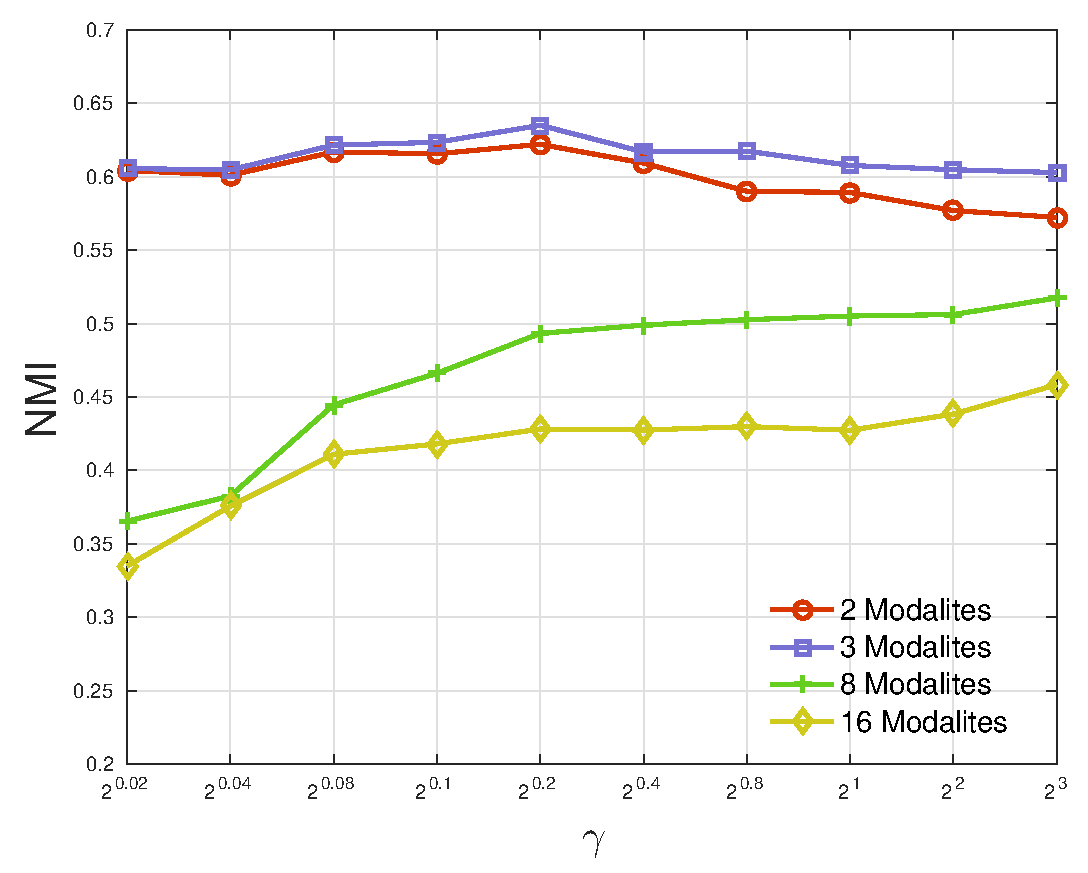
\includegraphics[width=0.49\textwidth]{chap3/corel_RWC_nmi.eps}
                    \label{fig3:rwc_corel}}
	\bisubcaptionbox{PASCAL VOC'07数据集}%
					{PASCAL VOC'07 dataset}
					[0.49\textwidth]{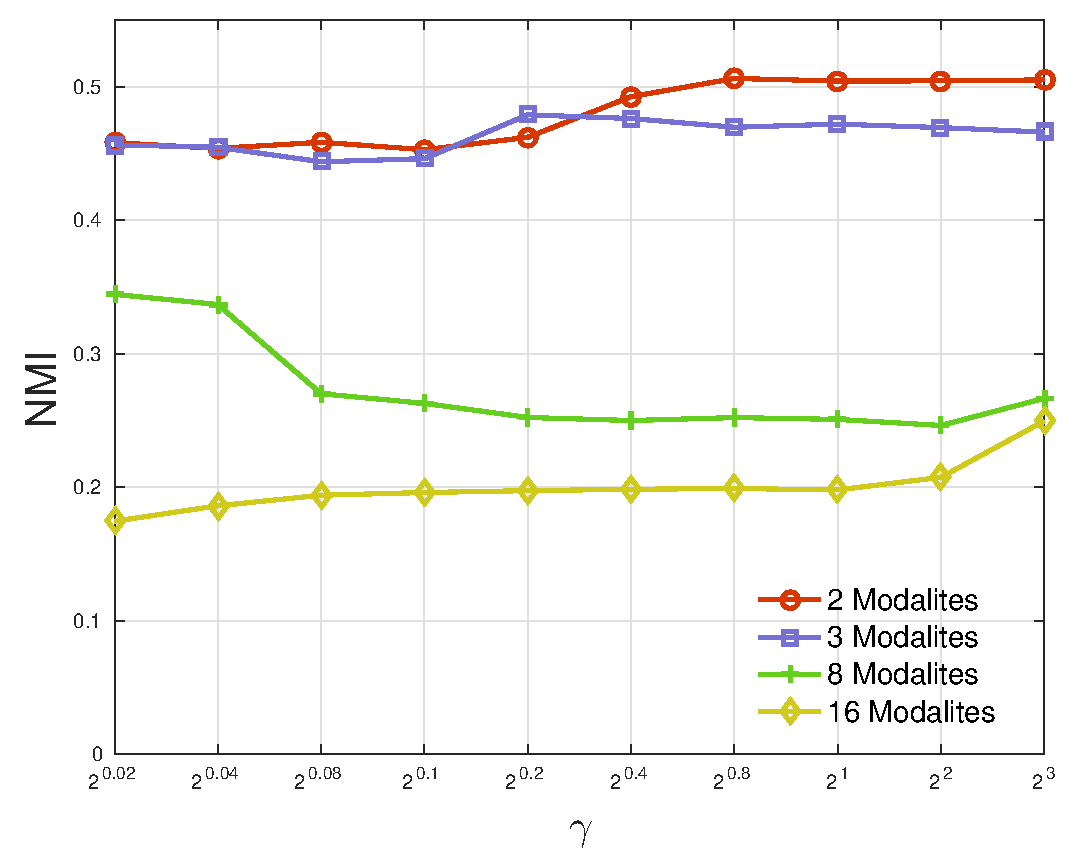
\includegraphics[width=0.49\textwidth]{chap3/voc_RWC_nmi.eps}
                    \label{fig3:rwc_voc}}
	\bicaption{在Corel 5k数据集和PASCAL VOC'07数据集上,超参数$\gamma$在不同的模态数量下对约束聚类效果的影响}{The influence of $ \gamma $ on Corel 5k and PASCAL VOC'07 datasets with different number of  modalities}
	\label{fig3:rwc}
\end{figure}

RWC方法在多模态聚类和多模态标签传播问题较为普遍\cite{wang2009unified,xu2016discriminatively,xu2014multi}。 在通用的标签传播框架内,RWC方法可以被描述为以下优化问题:
\begin{equation}
\begin{split}
\mathop{\mathrm{min}}_{{f},{\alpha}}\;g({f},{\alpha})=&\frac{1}{2}\eta\; \|{f}-{y}\|^2_2+\frac{1}{2}{f}^T \sum_s(\alpha_s)^\gamma{\bar{{L}}}_s{f}, \\
s.t. \quad&\sum_s \alpha_s = 1;\\
&\;\alpha_s \ge 0,
\end{split}
\label{eq3:labelpro}
\end{equation}
此处,向量$ {y} \in  \mathbb{R}^{n} $为观测到的类标签信息,向量$ {\alpha} \in  \mathbb{R}^m$为可学习的模态权重($m$为不同的模态数量),$ {f} \in  \mathbb{R}^{n}$为标签传播的估计结果,$ \gamma > 1$ 和$ \eta $ 是手动设定的参数。拉普拉斯矩阵$ \bar{{L}}_s $ 由公式(\ref{eq3:jointW})中的 $ \bar{{W}}_s $  及其相应的对角权重矩阵 $ \bar{{D}}_s $生成。在固定$f$的情况下,可以忽略公式(\ref{eq3:labelpro})中的第一项,并通过拉格朗日函数求解$ {\alpha} $
\begin{equation}
L({\alpha})=\sum_s(\alpha_s)^\gamma{f}^T {\bar{{L}}}_s{f} - \lambda ( \sum_s \alpha_s - 1)-\sum_s \mu_s \alpha_s,
\label{eq3:labelpro_L}
\end{equation}
其中$\lambda$和$\mu_s$为拉格朗日乘子,并且有$ \mu_s \ge 0$,$ \mu_s\alpha_s=0$。令函数(\ref{eq3:labelpro_L})对$ \alpha_s $的导数为零,能够得到
\begin{equation}
\gamma \alpha_s^{\gamma-1}{f}^T {\bar{{L}}}_s{f} =\lambda + \mu_s.
\label{eq3:labelpro_L_der}
\end{equation}
需要注意的是,为满足$ \mu_s\alpha_s=0 $,对于全部的$s$需要有$\mu_s=0 $。下文中将给出简要证明。

\begin{proposition}
   \label{thm3} 
    公式(\ref{eq3:labelpro_L_der})中,$\forall s \in \{1,\dots,m\}, \; \mu_s=0$。
\end{proposition}

\begin{proof}
    根据公式(\ref{eq3:labelpro_L})的约束条件已知$ \forall s \in \{1,\dots,m\}, \;\mu_s \ge 0$成立。

    现假设$\exists s \in \{1,\dots,m\}, \; \mu_s>0 $。由$ \mu_s\alpha_s=0 $可知必有$\alpha_s=0 $成立。
    则根据公式(\ref{eq3:labelpro_L_der})可知$\lambda + \mu_s = 0 $成立且$ \lambda<0 $成立。
    由于拉普拉斯矩阵$ {\bar{{L}}}_s $恒为半正定矩阵\cite{chung1997spectral},可知公式(\ref{eq3:labelpro_L_der})中$\forall s \in \{1,\dots,m\}, \;{f}^T {\bar{{L}}}_s{f} \ge 0$,即有$\forall s \in \{1,\dots,m\}, \; \lambda + \mu_s \ge 0 $。故:
    \begin{equation}
        \begin{split}
        \exists s \in \{1,\dots,m\}, \; \mu_s>0\; &\Rightarrow \;\lambda<0 \\&\Rightarrow \;\forall s \in \{1,\dots,m\}, \; \mu_s>0 \\&\Rightarrow \; \forall s \in \{1,\dots,m\}, \;\alpha_s=0.     
        \end{split}
    \end{equation}

    根据公式(\ref{eq3:labelpro_L})的约束条件$ \forall s \in \{1,\dots,m\}, \;\sum_s \alpha_s = 1$可知$ \exists s \in \{1,\dots,m\}, \;\alpha_s>0$,与假设产生矛盾,所以可知假设不成立,即有$\forall s \in \{1,\dots,m\}, \; \mu_s=0 $
\end{proof}

将公式(\ref{eq3:labelpro_L_der})代入约束条件 $ \sum_s \alpha_s=1 $ 可以得到
\begin{equation}
\alpha_s = \frac{({f}^T \bar{{L}}_s{f})^\frac{1}{1-\gamma}}{\sum_s({f}^T \bar{{L}}_s{f})^\frac{1}{1-\gamma}}.
\end{equation}

不同于线性组合权重$ \alpha_s$, 模态的权重系数被松弛为指数形式 $ \alpha_s^\gamma $ 以避免求得平凡解使得 $ {\alpha} $中仅有一个元素为 $ 1 $ 其他元素全部为 $ 0 $。

值得注意的是,在约束传播中,存在两个待优化函数。最理想化的方法是将公式(\ref{eq3:sol-v})中的$ {F}_v $看作是权重系数$\alpha$的一个函数,并用这个函数替换优化问题(\ref{eq3:MMCP-h})中的约束矩阵$Y$,以求解权重系数$\alpha$的最优解。将计算代价纳入考虑范围后,通过优化问题(\ref{eq3:baselinev})和(\ref{eq3:baselineh})来近似原优化问题的最小化子(minimizer),在其中我们不通过$F_v$和$F_h$来区分竖直传播和水平传播的结果,统一采用$F$表示传播结果,仅使用目标函数$g_v({F})$和$g_h({F})$来区分竖直传播和水平传播过程。

\begin{equation}
\mathop{\mathrm{min}}_{{F}}\;g_v({F})=\frac{1}{2}\eta\;\mathrm{tr}(({F}-{Y})^T\bar{{D}}({F}-{Y}))+\frac{1}{2}\mathrm{tr}({F}^T \sum_s(\alpha_s^{old})^\gamma\bar{{L}}_s{F}).
\label{eq3:baselinev}
\end{equation}

\begin{equation}
\begin{split}
\mathop{\mathrm{min}}_{{F},{\alpha}}\;g_h({F},{\alpha})&=\frac{1}{2}\eta\;\mathrm{tr}(({F}-{Y})\bar{{D}}({F}-{Y})^T)+\frac{1}{2}\mathrm{tr}({F} \sum_s(\alpha_s)^\gamma\bar{{L}}_s{F}^T), \\
s.t.\quad\;& \sum_s \alpha_s = 1;\\ & \; \alpha_s \ge 0.
\end{split}
\label{eq3:baselineh}
\end{equation}

假设公式(\ref{eq3:baselinev})中的权重系数为固定的常数向量,用$ {\alpha}^{old} $表示,而只通过优化问题(\ref{eq3:baselineh})更新权重系数,即$\alpha$。通过将向量$\alpha$的值赋给$ {\alpha}^{old} $,可以迭代地求解权重系数和约束传播结果$F$。

在固定$\alpha$的情况下,先求解公式(\ref{eq3:baselinev})并将其最优解作为$Y$带入公式(\ref{eq3:baselineh}),可求得$F$为
\begin{equation}
{F} = \eta^2(\eta\bar{{D}}+\bar{{L}})^{-1}\bar{{D}} {Y}\bar{{D}}(\eta\bar{{D}}+\bar{{L}})^{-1}, 
\label{eq3:bl_F}
\end{equation}
其中$\bar{{D}} = \sum_s (\alpha_s^{old})^\gamma  \bar{{D}}_s $ 且 $  \bar{{L}} = \sum_s (\alpha_s^{old})^\gamma  \bar{{L}}_s $,这与公式( \ref{eq3:unifiedW})相似。

在固定$F$的情况下,由公式(\ref{eq3:baselineh})可求得$\alpha$为
\begin{equation}
\alpha_s = \frac{\mathrm{tr}({F} \bar{{L}}_s{F}^T)^\frac{1}{1-\gamma}}{\sum_s \mathrm{tr}({F} \bar{{L}}_s{F}^T)^\frac{1}{1-\gamma}}, 
\end{equation}
并且更新${\alpha}^{old}$:$ {\alpha}^{old} \leftarrow {\alpha}$。由于根据公式(\ref{eq3:bl_F})计算出的$F$为对称矩阵,因此从竖直传播或水平传播中学习权重系数在结果上是等价的。

从公式(\ref{eq3:baselinev})和公式(\ref{eq3:baselineh})中,可以观察到超参数$ \gamma $在RWC方法中起到核心作用。每个模态的权重系数受$ \gamma $控制。 特别地,当$ \gamma \rightarrow \infty$时,该算法将生成全部相等的权重。而当 $ \gamma $趋近于 $ 1 $时,该算法将只选择一个具有最优一致性的模态,即令$  \mathrm{tr}({F} \bar{{L}}_s{F}^T) $最小的模态。我们在Corel 5k数据集和PASCAL VOC' 07数据集上,评估了超参数$\gamma$对在不同的模态数量下对约束聚类效果的影响。图\ref{fig3:rwc}展示了RWC方法在不同的$\gamma$取值情况下的约束聚类性能评估结果。我们可以观察到,当有极多模态数量的情况下,例如16个模态,RWC方法很难针对每个模态生成合适的权重。因而,当有16个模态时,RWC方法在$ \gamma = 2^3 $处取得最佳性能,此时各个模态的权重几乎相等。此外,图\ref{fig3:rwc}还显示$\gamma$的最佳选择在不同的数据集和不同数量的模态的情况下有所不同,很难选择可以广泛使用的$\gamma$值。在第\ref{sec3:exp}节的实验结果评估中,将选择在图\ref{fig3:rwc}中给出最优表现的$ \gamma $值,这一点与许多先前文献中的工作一样。然而,在实际的半监督问题中,这样的超参数选择策略往往是不可行的,因为经常没有足够标注数据可以作为验证集进行参数选择。

图\ref{fig3:cvg}给出了RWC方法的收敛曲线。可以看出优化问题的近似,公式(\ref{eq3:baselinev})和公式(\ref{eq3:baselineh}),能够在两到三次迭代后相对收敛。在第\ref{sec3:opt}节将给出更多的收敛性讨论。

\begin{figure}[t]
	\centering
	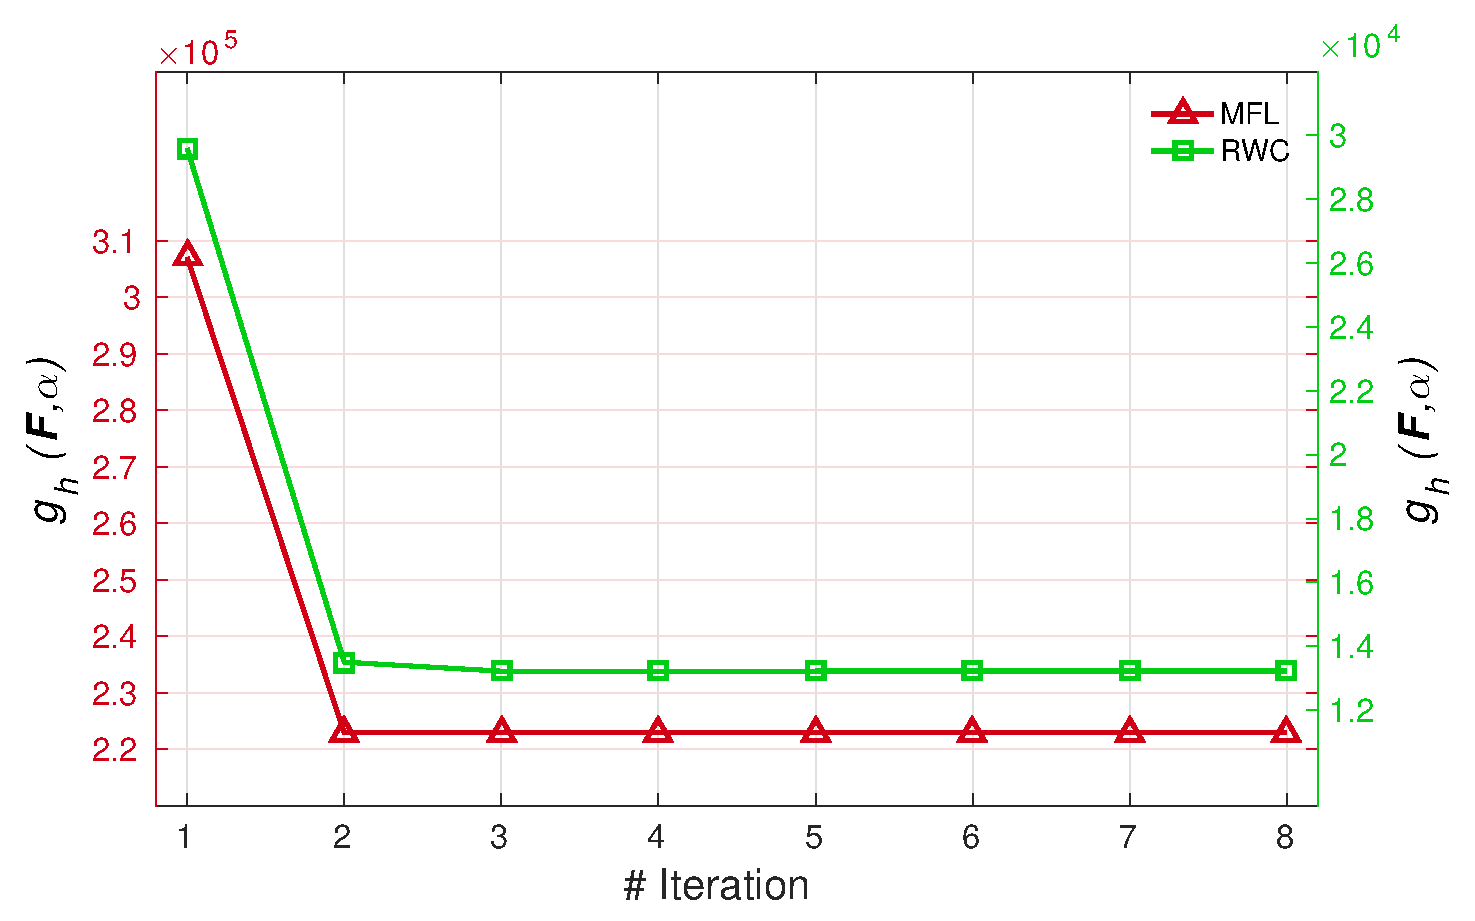
\includegraphics[width = 0.9\columnwidth]{chap3/cvg.eps}
	\bicaption{所提出的RWC方法和MFL方法在Corel 5k数据集上的收敛曲线}{The convergence curve of the proposed RWC and MFL on Corel 5k dataset.}
	\label{fig3:cvg}
\end{figure}

\subsection{多模态融合学习的公式化}
所提出的多模态融合学习(Multi-modal Fusion Learning,MFL)方法基于以下假设:在使用完美的权重系数的情况下,可以从每种模态的相似性矩阵中以最小的损失重建出观察到的约束。 换句话说,我们可以将数据中的成对约束视为每个模态的相似性的凸组合。而在观察到一部分成对约束的情况下,即已知约束矩阵$Y$,可以通过回归的方式来重构其他未观察到的约束。

基于这样的假设,我们将重构误差引入多模态约束传播的框架中。
假设在矩阵$Y$中有$l$个观测到的成对约束,即$Y$中有$l$个非零元素。然后可以对这$l$个不同的约束进行编号。定义两个函数$ r(i) $ 和 $ c(i) $,其中$ r(i) $ 的函数值为编号为$i$的约束在矩阵$Y$中的行号,函数$ c(i) $的值为相应的列号($i \in \{1,\dots,l\}$)。
则可以通过元素$ y_{r(i),c(i)} $对$Y$中的第$i$个约束进行定位和检索。基于这两个函数,可以构建约束向量$ {z} \in \mathbb{R}^n$:
\begin{equation}
z_i = \begin{cases}1,\quad\quad &\text{if}\;\; y_{r(i),c(i)} =1; \\
0, \quad\quad &\text{otherwise}.
\end{cases}
\end{equation} 
此处可理解为,must-link在向量$z$中对应$1$,cannot-link对应$0$,为观测到的约束不出现在约束向量$z$中。

同时可以根据所有模态的相似性矩阵$ \{{W}_s|s\in\{1,\dots,m\}\} $构建相应的基矩阵$ {S} \in \mathbb{R}^{l\times m}$($l$为约束的数量,$m$为模态数量),
\begin{equation}
 {S}_{i,s} = w_{r(i), c(i), s}.
\end{equation}
则重构误差可以定义为
\begin{equation}
error = \|{S}{\alpha}-{z}\|_2^2,
\end{equation}
这里 $ {\alpha} $ 为权重系数。
由于${W}_s$为稀疏的相似性矩阵,所以该重构误差可以理解为,对于相似性为$0$的点对关系应对应于向量$z$中的cannot-link值即$0$,而相似性大于$0$的点对关系对应于向量$z$中的must-link值即$1$。

需要引起注意的是,$z$中的must-link和cannot-link的比例大约为$1:c-1 $,其中$c$为类别数。如果从高度稀疏的相似性矩阵中生成矩阵 $S$,则在矩阵 $S$中会存在极大量的零元素,这将使得样本分布不均衡,重构变得很困难。所以与用于构造拉普拉斯矩阵$ \bar{{L}}_s $的高度稀疏的相似性矩阵不同,基矩阵$S$ 由近邻数为$ k=\frac{\#sample}{\#cluster} = \frac{n}{c}$ 的相对密集的相似性矩阵生成。在这种情况下 矩阵$S$ 和 向量$z$中零元素与非零元素的比例大致相似。

将重构误差纳入考虑范围后,可以设计出一个优化问题以同时最小化传播误差和重构误差。与RWC方法中的近似方式相似,我们仅从水平方向的约束传播学习权重系数,从而可以得出以下优化问题:

\begin{equation}
\mathop{\mathrm{min}}_{{F}}\;g_v({F})=\frac{1}{2}\eta \;\mathrm{tr}(({F}-{Y})^T\bar{{D}}({F}-{Y}))+\frac{1}{2}\mathrm{tr}({F}^T \sum_s\alpha_s^{old}\bar{{L}}_s{F}),
\label{eq3:MFL_v}
\end{equation}
及
\begin{equation}
\begin{split}
\mathop{\mathrm{min}}_{{F},{\alpha}}\;g_h({F}, {\alpha})=&\frac{1}{2}\eta\;\mathrm{tr}(({F}-{Y})\bar{{D}}({F}-{Y})^T)+\frac{1}{2}\mathrm{tr}({F} \sum_s\alpha_s\bar{{L}}_s{F}^T) \\ &+\frac{1}{2}\zeta\|{S}{\alpha} - {z}\|_2^2,\\
s.t. \quad\;& \sum_s \alpha_s = 1;\\ &\; \alpha_s \ge 0.
\end{split}
\label{eq3:MFL}
\end{equation}

在公式(\ref{eq3:MFL})中,我们采用了与E$^2$CP\cite{lu2010constrained} 和MMCP\cite{fu2011multi}方法中相同的$ \eta $取值,即$ \eta = 0.25 $,并且将竖直方向的传播问题(\ref{eq3:MFL_v})的最优解作为水平方向传播约束矩阵 $ {Y} $。至于参数 $ \zeta $,我们认为在重构误差中的元素应该与$ \mathrm{tr}({F} \sum_s\alpha_s\bar{{L}}_s{F}^T) $中的元素具有相似的重要性。 如果将$ \sum_s\alpha_s\bar{{L}}_s $ 看作一个距离度量矩阵,则$ \mathrm{tr}({F} \sum_s\alpha_s\bar{{L}}_s{F}^T) $ 可以认为时投影后的$ {F}^T $的Frobenius 范数的平方,即是$\#sample^2=n^2$个元素的平方和。同时,重构误差也可以被看作是一个Frobenius范数平方的特例,其中包含了$ \#constraint = l $ 个元素。所以选择 $ \zeta = \frac{\#sample^2}{\#constraint}=\frac{n^2}{l} $使这两项处于同一重要性级别。

公式(\ref{eq3:MFL})可以利用观察到的成对约束来学习权重系数,而不是仅仅从与约束传播相同的优化目标函数中学习一个比率。使用更多的观察到的信息将能够提高所提出的方法的鲁棒性。通过组合重构误差和约束传播误差,多模态约束传播的目标函数不再是单模态约束传播目标函数的简单组合,并且不会出现第\ref{sec3:rwc}节中提到的平凡解,因此也不需要采用指数形式对权重系数进行松弛。

\subsection{多模态融合学习的优化}
\label{sec3:opt}

\begin{algorithm}[t]
	\SetKwInput{KwData}{输入}
    \SetKwInput{KwResult}{输出}
	\caption{多模态融合学习}
	\label{alg3:MFL}
	\KwData{相似性矩阵 $W_s$;约束矩阵$Y$;基矩阵 $S$;聚类数量$c$。}
    \KwResult{统一的相似性矩阵 $W^*$。}
    选择初始化的可行权重参数向量$ {\alpha}^0_0 $,$ i = 0 $;\\
    \Repeat{收敛}{
        根据公式(\ref{eq3:MFL_F})计算$ {F}_{i+1} $。\\
        选择初始化的乘子$ \lambda_0 $ 和惩罚参数$ \mu_0 $; 初始化$ \varepsilon_0 > 0 $; $ j = 0 $;\\
        \Repeat{收敛}{
            通过投影梯度法近似求解公式(\ref{eq3:MFL_L})${\alpha}^i_j =  \mathrm{arg}\mathop{\mathrm{min}}\limits_{{\alpha}}\;\mathcal{L}({\alpha},\lambda_j;\mu_j)$;\\                        
            \uIf{$ \|\mathbf{1}^T{\alpha}_j^i- 1\| \le \varepsilon_j $}{
                $ \lambda_{j+1} \leftarrow \lambda_j - \mu_j(\mathbf{1}^T{\alpha}_j^i- 1) $;\\
                $ \mu_{j+1} \leftarrow \mu_j $;\\
                $ \varepsilon_{j+1} \leftarrow \varepsilon_j \mu^{-0.9 }$;\\
            }
            \Else{
                $ \lambda_{j+1} \leftarrow \lambda_j$;\\
                $ \mu_{j+1} \leftarrow 100\mu_j $;\\
                $ \varepsilon_{j+1} \leftarrow \mu^{-0.1 }$;\\
            }

            $ j\leftarrow j+1 $;\\
        }
        $ i\leftarrow i+1 $;\\
    }
    根据公式(\ref{eq3:rSa}),通过整流Sigmoid激活函数,由$F_i$生成$W^*$。
\end{algorithm}

MFL方法的求解可以分解为两个子问题,并能够通过交替迭代法求解。在本节中,我们将描述优化求解过程的一些细节。

    \textbf{固定$\alpha$求解$F$}:

当权重系数$\alpha$固定时,公式(\ref{eq3:MFL})可以被化简为公式(\ref{eq3:MMCP-h})。因此,我们可以发现$F$的解与公式(\ref{eq3:bl_F})非常相似:
\begin{equation}
{F} = \eta^2(\eta\bar{{D}}+\bar{{L}})^{-1}\bar{{D}} {Y}\bar{{D}}(\eta\bar{{D}}+\bar{{L}})^{-1},
\label{eq3:MFL_F}
\end{equation}
在其中$  \bar{{D}} = \sum_s \alpha_s  \bar{{D}}_s $ and $  \bar{{L}} = \sum_s \alpha_s \bar{{L}}_s $

    \textbf{固定$F$求解$\alpha$}:

当$F$固定时,公式(\ref{eq3:MFL})可以被变形为有界约束的二次优化问题(bound-constrained quadratic optimization problem):
\begin{equation}
\begin{split}
\mathop{\mathrm{min}}_{{\alpha}}\;&\frac{1}{2}\mathrm{tr}({F} \sum_s\alpha_s\bar{{L}}_s{F}^T)+\frac{1}{2}\zeta\|{S}{\alpha} - {z}  \|_2^2,\\
s.t.\quad& \sum_s \alpha_s = 1;\\ &\; \alpha_s \ge 0.
\end{split}
\label{eq3:MFL_ALM}
\end{equation}    
考虑到公式(\ref{eq3:MFL_ALM})的计算复杂度与$\alpha$的维度相关,即与模态数量相关,并且$\alpha$为低维向量,我们采用了增广拉格朗日方法\cite{bertsekas1982constrained}优化所提出的目标函数。
我们沿用了文献\parencite{nocedal2006numerical} 和文献\parencite{bertsekas1982constrained}中所介绍的有界约束拉格朗日优化方法(bound-constrained Lagrangian,BCL)的详细策略。通过将公式(\ref{eq3:MFL_ALM})中的等式约束纳入增广拉格朗日方法可以生成子问题
\begin{equation}
\begin{split}
\mathop{\mathrm{min}}_{{\alpha}}\;\mathcal{L}({\alpha},\lambda;\mu) =&\frac{1}{2}\zeta\|{S}{\alpha} - {z}\|_2^2+\frac{1}{2}\sum_s\alpha_s\mathrm{tr}({F} \bar{{L}}_s{F}^T) \\
&- \lambda(\mathbf{1}^T{\alpha}-1)+\frac{\mu}{2}(\mathbf{1}^T{\alpha}-1)^2\\
s.t.\quad &\alpha_s \ge 0.
\end{split}
\label{eq3:MFL_L}
\end{equation}
我们采用了投影梯度法(gradient projection method)对公式(\ref{eq3:MFL_L})中的子问题进行近似求解,然后更新乘子$ \lambda $ 和和惩罚系数 $ \mu $,并重复迭代该过程\cite{nocedal2006numerical,conn1992lancelot}。算法\ref{alg3:MFL}对所提出的方法以及后处理进行了总结。

图\ref{fig3:cvg}展示了MFL方法的收敛曲线。可以发现,一旦在RWC方法和MFL方法中将权重系数分解为$ {\alpha}^{old} $ 和 $ {\alpha} $两部分,$ {\alpha}^{old} $可以被看作为常数向量。然后,我们学习MMCP算法的做法,将水平方向约束传播目标函数(公式(\ref{eq3:baselineh})和公式(\ref{eq3:MFL}))中的约束矩阵$Y$代换为竖直方向约束传播所求得的最优解。通过代换,仅需要考虑更新传播结果$F$和系数$\alpha$。下文将简要论述该迭代算法的收敛性。

由于对角权重矩阵$ \bar{{D}}_s $和拉普拉斯矩阵$\bar{L}_s$都为半正定矩阵,其凸组合$ \sum_s\alpha_s\bar{{L}}_s $也为半正定矩阵。因此,公式(\ref{eq3:MFL})的目标函数中三项皆为为负值,且有$ g_h({F}, {\alpha}) \ge 0 $。我们可以通过任意可行解$F_0$对$F$的解集进行定界,以得到一个$(F, \alpha)$的紧致解集。例如,在原优化问题基础上增加一个辅助约束:
\begin{equation}
        \frac{1}{2}\eta\;\mathrm{tr}(({F}-{Y})\bar{{D}}({F}-{Y})^T)  \le g_h({F}_0, {\alpha}),
\end{equation}
并且优化问题(\ref{eq3:MFL})的最优解恒满足此辅助约束条件。极值定理(extreme value theorem)保证了从非空紧空间到一个实数子集的连续映射函数$ g_h({F}, {\alpha})$必然存在最优解$({F}^*, {\alpha}^*) $使得函数取得最小值。

更进一步地,原目标函数为分别关于$F$和$\alpha$的凸函数。对于一个迭代序列集合$ \{({F}^{(t)}, {\alpha}^{(t)})\} $,有
\begin{equation}
    g_h({F}^{(t)}, {\alpha}^{(t)}) \ge \mathop{\mathrm{min}}_{{F}} g_h({F}, {\alpha}^{(t)}) = g_h({F}^{(t+1)}, {\alpha}^{(t)}) \ge \mathop{\mathrm{min}}_ {{\alpha}} g_h({F}^{(t+1)}, {\alpha}) =g_h({F}^{(t+1)}, {\alpha}^{(t+1)}).
\end{equation}
所以,针对$F$和针对$\alpha$的迭代步骤都可以最小化目标函数(\ref{eq3:MFL}),这显示了所提出的RWC和MFL算法都可以有效收敛。如图\ref{fig3:cvg}所示,MFL算法可以在大约两轮迭代中近似收敛。

\subsection{后处理流程}
在先前关于约束传播的大多数工作中,传播结果$F$被用于完善原始$k$-NN相似性矩阵$W$:
\begin{equation}
w^*_{i,j} = 
\begin{cases}
1-(1-f_{i,j})(1-w_{i,j}), \qquad &f_{i,j}\ge 0;\\
(1+f_{i,j})w_{i,j}, &f_{i,j}< 0,
\end{cases}
\label{eq3:refine}
\end{equation}
其中,$ w_{i,j} $ 为数据实例 $ x_i $ 和$ x_j $之间的相似性。

上述通过调整获得最终解的方法有两个不足之处。一方面,传播结果$ {F} $的信息未被充分利用。另一方面,求得的最终结果高度取决于原始相似性矩阵的质量。在我们的RWC和MFL方法中,我们放弃了原始的相似性矩阵,而采用整流Sigmoid激活函数从从$F$中直接生成统一的相似性矩阵:
\begin{equation}
w^*_{i,j} = 
\begin{cases}
\frac{1}{1+\text{exp}(-f_{i,j}/\sigma)}, \qquad &\text{if }f_{i,j}>0;\\
0, &\text{otherwise, }
\end{cases}
\label{eq3:rSa}
\end{equation}
在这里,$ \sigma  $为矩阵$F$中所有元素的强度的均值。整流Sigmoid函数使得统一的相似性矩阵完全依赖于传播的结果。此外,使用整流Sigmoid函数比完善方法更具有可解释性。对于传播结果$F$中的正元素,Sigmoid函数部分将传播结果的数值投影到$0.5$到$1$之间,这可以被解释为一个联合概率。对于负元素,负值表示两个数据样本被预测为不属于同一个类别。因此,我们根据$k$-NN热力核的定义,在统一相似性矩阵中将这些约束设置为$0$,而不是通过Sigmoid函数得到一个正值的相似性。

随后,我们对$ W^* $应用谱聚类方法\cite{von2007tutorial}进行特征投影,并通过$ k$-means聚类对结果进行评估。

\subsection{权重系数的稀疏性}
\label{sec3:dis}
如果基矩阵$S$的列向量线性无关,我们可以将矩阵$S$的左逆矩阵表示为$ {S} ^+ = ({S}^T{S})^{-1}{S}^T$。定义向量 $ {h} \in  \mathbb{R}^{m} $为
\begin{equation}
h_s = \text{tr}({F} \bar{{L}}_s{F}^T).
\end{equation}
我们可以将优化问题(\ref{eq3:MFL_ALM})变形为
\begin{equation}
\begin{split}
\mathop{\mathrm{min}}_{{\alpha}}\;&\|{S}{\alpha} - ( \mathbf{z} - \frac{1}{2\zeta}{S}^+ {h}) \|_2^2,\\
s.t.\quad& \sum_s \alpha_s = 1;\\ &\; \alpha_s \ge 0.
\label{eq3:nnls}
\end{split}
\end{equation}

公式(\ref{eq3:nnls})是一个在凸约束$ \sum_s \alpha_s = 1 $下的非负最小二乘法(non-negative least square,NNLS)问题的特例。在我们所提出的MFL可以观察到一些NNLS问题的特性。
在回归系数上的非负约束具有与显式的稀疏正则化项相似的效果,并且NNLS有与LASSO \cite{tibshirani1996regression}相当的稀疏性能,这一点在文献\parencite{slawski2011sparse}和文献\parencite{slawski2013non}中都有进一步的论证,并且在我们的实验中也能够观察到这种性质。随着我们为所提出的算法提供更多的模态信息,权重系数的稀疏性变得更加明显。当我们在8种不同模态上应用所提出的方法时,我们注意到大约有2或3个模态的权重为零。当我们使用的模态数达到16个时,将有大约一半的零权重。因此,MFL可以用作模态选择器,并且仅在候选列表中保留有帮助的模态。这也是当存在极多不同模态是时我们的方法具有鲁棒表现的主要原因。

\begin{table}[tb]
	\bicaption{在Corel 5k和PASCAL VOC'07数据集上采用2种模态情况下的聚类性能}{Clustering performance of 2 modalities on Corel 5k and PASCAL VOC'07}
	\label{tab3:2modal}
	\centering
	\setlength{\tabcolsep}{15pt}
	\begin{tabular}{lcccc}
		\toprule
		&\multicolumn{2}{c}{Corel 5k} & \multicolumn{2}{c}{PASCAL VOC'07} \\
		\cmidrule(lr){2-3}
		\cmidrule(lr){4-5}
		& ACC\% & NMI\% & ACC\% & NMI\% \\
		\midrule
		NCuts\cite{shi2000normalized} & 40.23 & 50.68 & 34.11 & 36.06 \\ 
		E$^2$CP\cite{lu2010constrained} & 49.76 & 59.05 & 46.84 & 45.26 \\
		MCMCP\cite{fu2012modalities} & 50.20 & 60.42 & 46.00 & 44.13 \\  
		MMCP\cite{fu2011multi} & 43.22 & 53.10 & 51.42 & 46.99 \\ 
		UCP\cite{lu2013unified} & 48.98 & 59.39 & 36.43 & 24.31 \\ 
		MSCP\cite{lu2013exhaustive} & 50.18 & 60.74 & 37.33 & 32.82 \\ 
		\midrule
		SW & 48.44 & 56.33 & \textbf{57.44} & \textbf{50.28} \\ 
		RWC & \textbf{54.97} & 62.11 & 56.80 & 50.24 \\ 
		MFL & 54.87 & \textbf{62.32} & 55.07 & 48.55 \\ 
		\bottomrule
	\end{tabular}
\end{table}


\section{实验结果}
\label{sec3:exp}
在本节中,我们报告一些实验结果以证明所提出的MFL方法和基线方法RWC的有效性。我们在两个公开可用的数据集上进行了大量的约束聚类实验,展示了所提出的方法在不同的模态数量下的聚类性能及其模态选择能力。

\subsection{数据集描述}
在我们的实验中,我们采用了INRIA\footnote{\url{http://lear.inrialpes.fr/people/guillaumin/data.php}}发布的两个被广泛使用的多模态特征数据集\cite{guillaumin2009tagprop}:
\begin{itemize}
    \item {\textbf{Corel 5k}}。Corel 5k自然图像数据集是一个重要的基准数据集,在许多不同任务上被广泛采用。Corel 5k具有50个类别和4999张自然图像。数据集中的每张图像都有一组关键字描述,这些关键词选取自一个包含260个单词的关键词词典。
    \item {\textbf{PASCAL VOC'07}}。PASCAL VOC'07数据集\cite{pascal-voc-2007}包含20个图像类别和9963张图像。据集中的所有图像均带有一个或多个类别标注。文字描述基于一个包含804个关键词的词典。
\end{itemize}

INRIA特征数据集\cite{guillaumin2009tagprop}对Corel 5k和PASCAL VOC'07数据集中的图像进行了相同标准的特征抽取,分别生成了一个多模态特征数据集。对于每一个数据集,INRIA特征中包含了16中不同的特征,其中包含了15种视觉特征(1种Gist特征,6种颜色直方图特征和8种词袋特征):\textit{DenseSift,DenseSiftV3H1,HarrisSift,HarrisSiftV3H1,DenseHue,DenseHueV3H1,HarrisHue,HarrisHueV3H1,Rgb,RgbV3H1,Lab,LabV3H1,Hsv,HsvV3H1,Gist}。以及1种关键词表述特征:\textit{tag}。
此外,为多模态半监督学习任务而创建的这些特征数据集也可以被视为多模态多视图数据集,在我们的实验中,我们将每种特征视为一个独立的模态。

\subsection{对照算法介绍}
我们将我们所提出的MFL和RWC算法和一些在第\ref{sec3:intro}节种提及的目前先进的方法以及部分基线方法进行了比较。
以下是我们在实验中所用于对比的算法:
\begin{itemize}
    \item {\textbf{MMCP}}。正如在\ref{sec3:intro}中所提到的那样,由于在半监督聚类问题的设置中,很难手动确定每个模态的重要性。在我们的实验中,我们为MMCP\cite{fu2011multi}中的每个模式设置了同等的重要性。
    \item {\textbf{SW}}。SW(same weight)是本文提出的另一个基线方法,表示所有模态具有的权重相同。在SW中,我们删除了MFL中的权重学习步骤,并强制每个模态具有相同的权重。在我们的实验中,SW方法与MMCP算法相似。它们之间的唯一区别在于,SW采用了整流Sigmoid激活函数来生成最终的相似性矩阵,而MMCP采用了公式(\ref{eq3:refine})中调整完善的方法。
    \item {\textbf{MSCP}}。Multi-Source Constraint Propagation(MSCP)\cite{lu2013exhaustive}方法专注于两种模态上的的约束传播。在本节中,我们将在两种模态的情况下将我们的方法与MSCP进行比较。
    \item {\textbf{UCP}}。Unified Constraint Propagation(UCP)\cite{lu2013unified}方法同时进行了视图内和视图间的约束传播,这种方法同样是针对两种模态的情况所设计的。
    \item {\textbf{MCMCP}}。Modalities Consensus for Multi-modal Constraint Propagation(MCMCP)\cite{fu2012modalities}方法通过迭代法求解约束传播问题。在每一行迭代中,MCMCP方法会在每一个模态上分别进行一次传播,这使得整个算法非常耗时。
    \item {\textbf{E$^2$CP}}。E$^2$CP\cite{lu2010constrained}方法是一个单模态约束传播方法,但我们依然将该方法引入我们的实验中作为一个基线方法。在我们的实验中,我们在每个模态上单独使用E$^2$CP,然后将算法在每个模态上生成的经传播调整完善后的相似性矩阵求平均,以此作为多模态的E$^2$CP方法结果。
    \item {\textbf{NCuts}}。在实验中,我们报告了没有传播过程而仅采用Normalized Cuts(NCuts)\cite{shi2000normalized}的聚类结果作为参考。在对NCuts算法进行实验时,我们用相同的权重对各模态的相似性矩阵取平均值。
\end{itemize}

\subsection{实验设置}
\begin{table}[t]
	\bicaption{在Corel 5k数据集上采用3个、8个和16个模态的聚类性能}{Clustering performance of 3, 8 and 16 modalities on Corel 5k.}
	\label{tab3:modal_corel}
	\centering
	\setlength{\tabcolsep}{8pt}
	\begin{tabular}{l*{6}{c}}
		\toprule
		&\multicolumn{2}{c}{3 modalities} & \multicolumn{2}{c}{8 modalities} & \multicolumn{2}{c}{16 modalities} \\
		\cmidrule(lr){2-3}
		\cmidrule(lr){4-5}
		\cmidrule(lr){6-7}
		& ACC\% & NMI\% & ACC\% & NMI\% & ACC\% & NMI\% \\
		\midrule
		NCuts\cite{shi2000normalized} & 44.98 & 54.33 & 38.61 & 49.27 & 32.07 & 42.11 \\ 
		E$^2$CP\cite{lu2010constrained} & 52.64 & 61.14 & 40.19 & 50.17 & 28.80 & 39.17 \\ 
		MCMCP\cite{fu2012modalities} & 49.15 & 59.90 & 36.72 & 51.56 & 36.24 & 51.12 \\ 
		MMCP\cite{fu2011multi} & 48.50 & 56.58 & 37.82 & 48.33 & 32.98 & 43.63 \\ 
		\midrule
		SW & 51.83 & 60.40 & 42.61 & 50.53 & 33.74 & 42.81 \\
		RWC & 55.51 & 63.44 & 43.60 & 51.60 & 36.56 & 45.43 \\
		MFL & \textbf{56.36} & \textbf{63.99} & \textbf{57.04} & \textbf{64.11} & \textbf{56.67} &\textbf{ 64.09} \\
		\bottomrule
	\end{tabular}
\end{table}

\begin{table}[t]
	\bicaption{在PASCAL VOC'07数据集上采用3个、8个和16个模态的聚类性能}{Clustering performance of 3, 8 and 16 modalities on PASCAL VOC'07.}
	\label{tab3:modal_voc}
	\centering
	\setlength{\tabcolsep}{8pt}
	\begin{tabular}{lcccccc}
		\toprule
		&\multicolumn{2}{c}{3 modalities} & \multicolumn{2}{c}{8 modalities} & \multicolumn{2}{c}{16 modalities} \\
		\cmidrule(lr){2-3}
		\cmidrule(lr){4-5}
		\cmidrule(lr){6-7}
		& ACC \% & NMI \% & ACC \% & NMI \% & ACC\% & NMI\%		\\
		\midrule 
		NCuts\cite{shi2000normalized} & 26.76 & 25.04 & 23.07 & 21.26 & 22.31 & 18.40 \\
		E$^2$CP\cite{lu2010constrained} & 40.46 & 39.50 & 29.39 & 26.40 & 25.66 & 21.29 \\ 
		MCMCP\cite{fu2012modalities} & 34.85 & 27.34 & 29.36 & 24.79 & 29.80 & 24.98 \\  
		MMCP\cite{fu2011multi} & 38.29 & 36.14 & 29.04 & 26.40 & 27.85 & 24.90 \\
		SW & 49.96 & 45.77 & 31.67 & 24.25 & 29.98 & 20.15 \\ 
		RWC & 53.27 & 47.55 & 42.07 & 34.33 & 29.08 & 24.97 \\ 
		MFL & \textbf{56.66} & \textbf{49.98} & \textbf{54.95} & \textbf{49.06} & \textbf{56.35} & \textbf{49.86} \\ 
		\bottomrule
	\end{tabular}
\end{table}
为了评估这些方法的聚类性能,我们在实验中采用准确率(accuracy,ACC)和归一化互信息(normalized mutual information,NMI)作为聚类结果的性能测度。
由于约束传播方法的性能在某种程度上取决于约束矩阵${Y}$的选择。我们在每个实验中生成多个约束矩阵,并在本节中报告算法在不同约束矩阵上的平均性能。
我们在$k$-means阶段部署30次聚类,并选择类内和最小的聚类结果作为$k$-means阶段的结果。


\begin{figure}[t]
	\centering
	\bisubcaptionbox{Corel 5k数据集上的ACC结果}%
					{ACC on  Corel 5k}
					[0.49\textwidth]{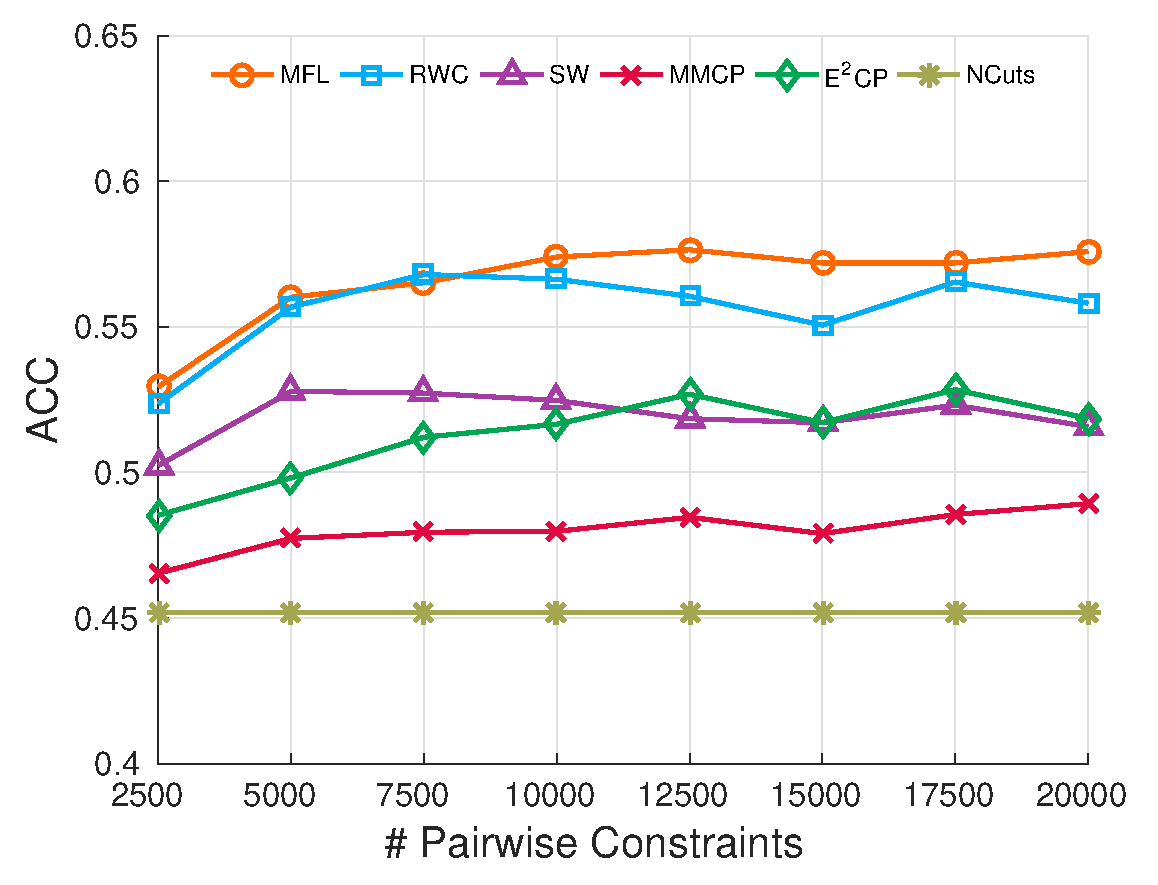
\includegraphics[width=0.49\textwidth]{chap3/corel5k_cn_acc.eps}}
                    \label{fig3:corel5k_cn_acc}
	\bisubcaptionbox{Corel 5k数据集上的NMI结果}%
					{NMI on  Corel 5k}
                    [0.49\textwidth]{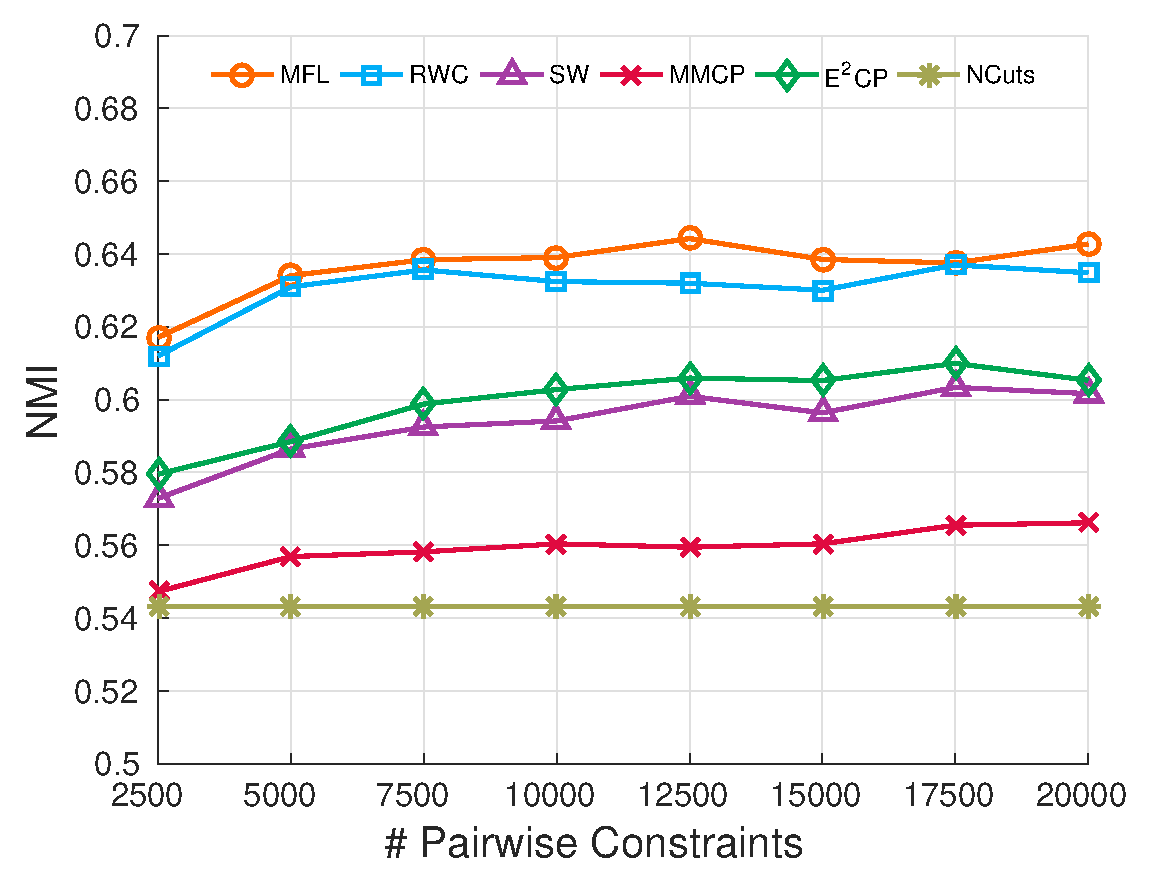
\includegraphics[width=0.49\textwidth]{chap3/corel5k_cn_nmi.eps}}
                    \label{fig3:corel5k_cn_nmi}
                    
	\centering
	\bisubcaptionbox{PASCAL VOC'07数据集上的ACC结果}%
					{ACC on  PASCAL VOC'07}
					[0.49\textwidth]{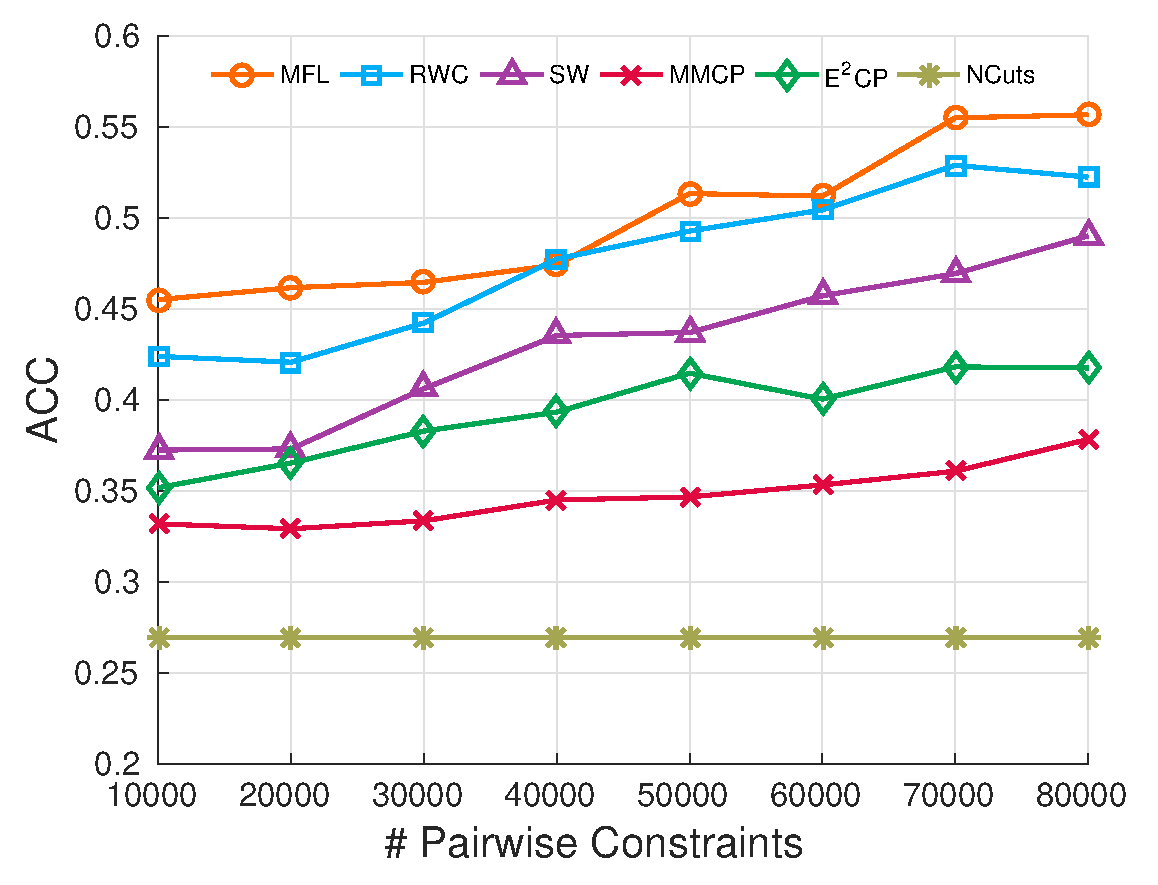
\includegraphics[width=0.49\textwidth]{chap3/voc_cn_acc.eps}}
                    \label{fig3:voc_cn_acc}
	\bisubcaptionbox{PASCAL VOC'07数据集上的NMI结果}%
					{NMI on  PASCAL VOC'07}
					[0.49\textwidth]{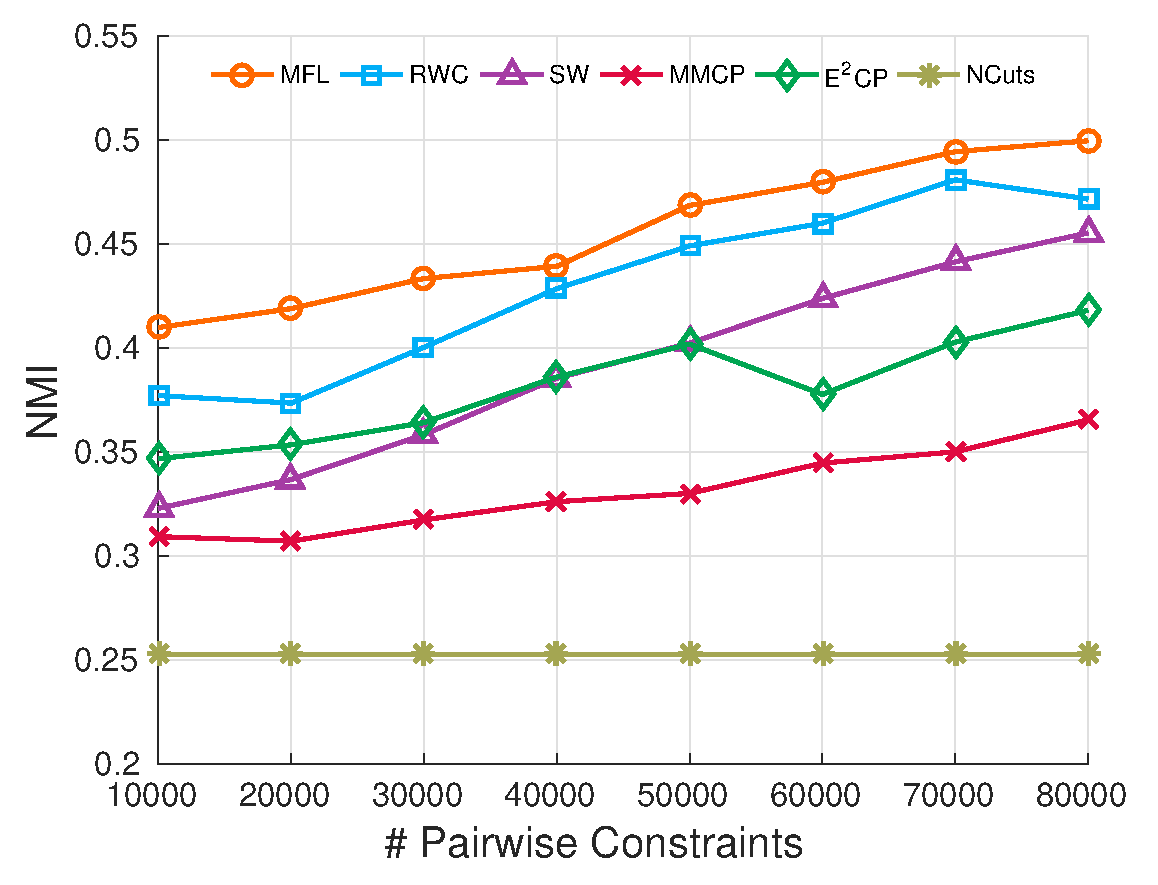
\includegraphics[width=0.49\textwidth]{chap3/voc_cn_nmi.eps}}
                    \label{fig3:voc_cn_nmi}
	\bicaption{在Corel 5k和PASCAL VOC'07数据集上,不同约束数量下采用3个模态的聚类效果}{Clustering performance of 3 modalities on Corel 5k and PASCAL VOC'07 with different numbers of  constraints}
	\label{fig3:cn}
\end{figure} 


\begin{figure}[t]
	\centering
	\bisubcaptionbox{Corel 5k数据集上的ACC结果}%
					{ACC on  Corel 5k}
					[0.49\textwidth]{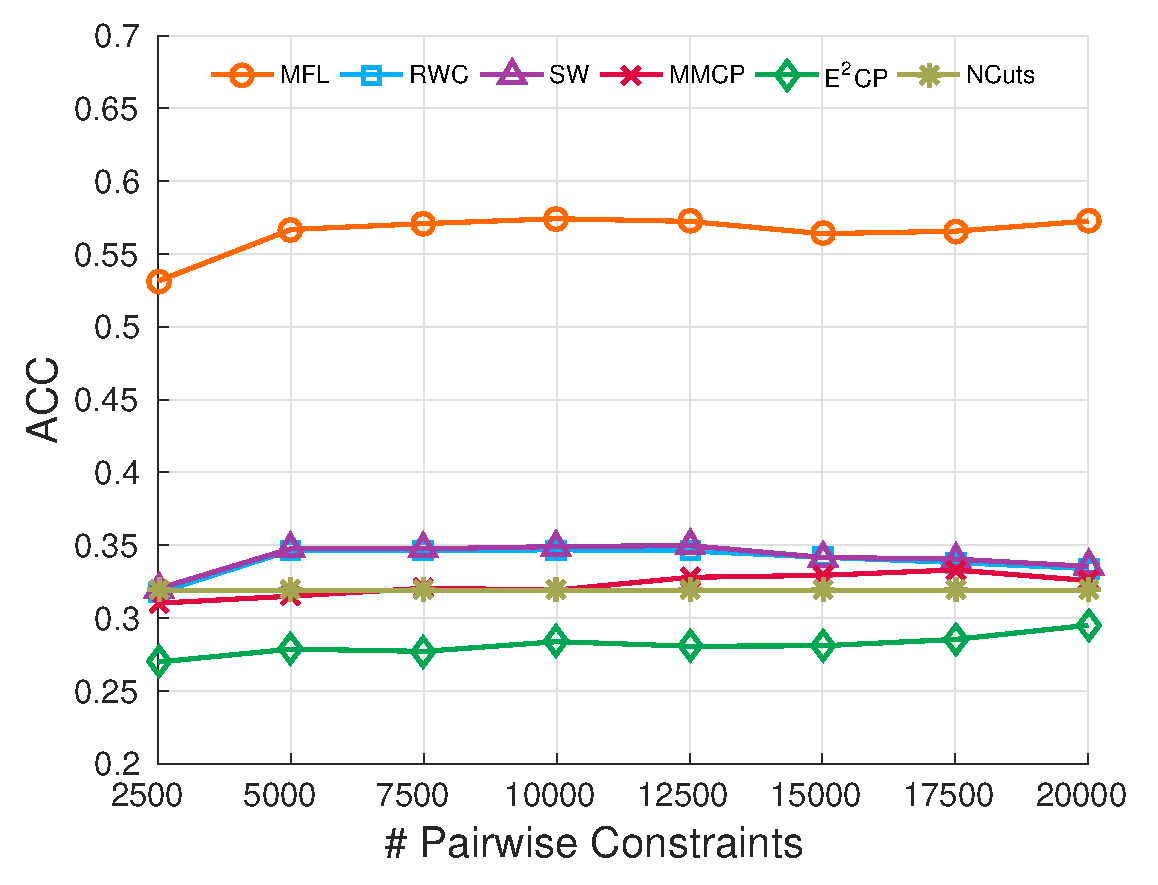
\includegraphics[width=0.49\textwidth]{chap3/corel5k_cn_16_acc.eps}}
                    \label{fig3:corel5k_cn_16_acc}
	\bisubcaptionbox{Corel 5k数据集上的NMI结果}%
					{NMI on  Corel 5k}
                    [0.49\textwidth]{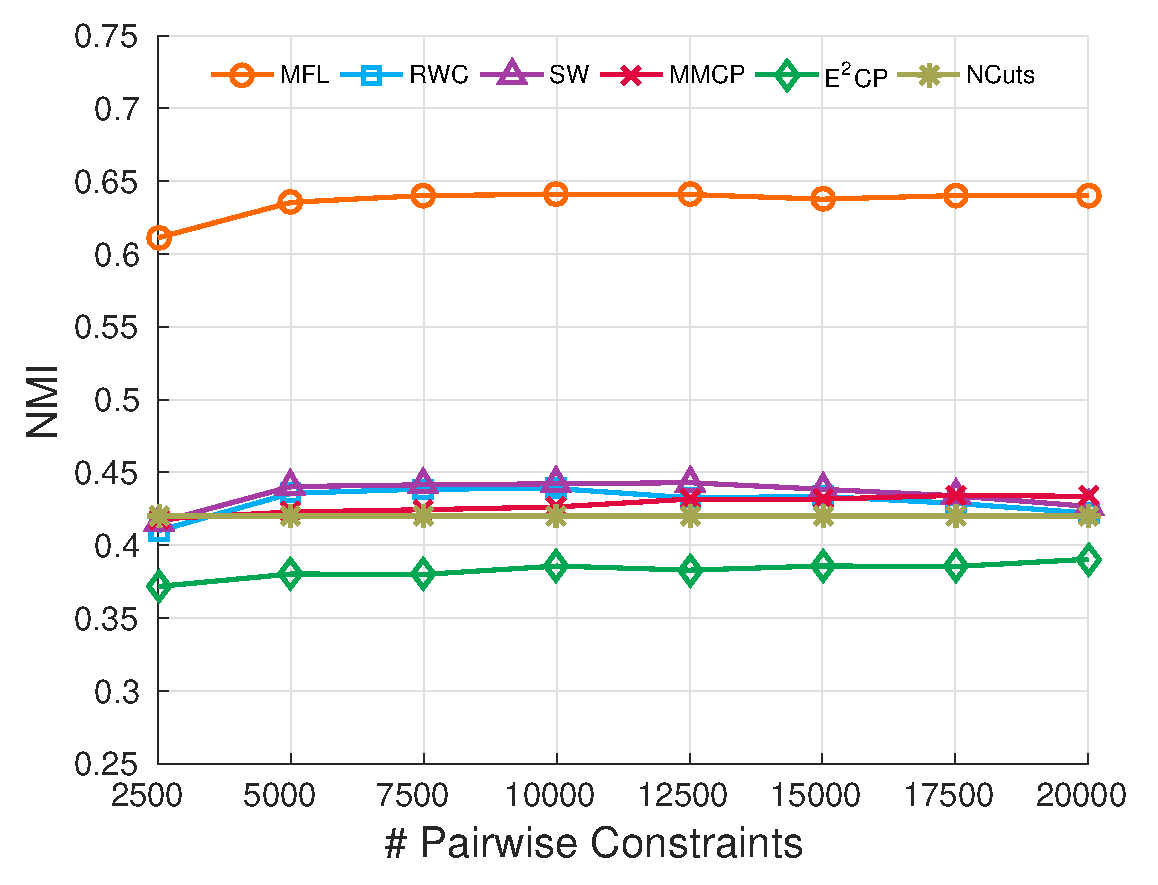
\includegraphics[width=0.49\textwidth]{chap3/corel5k_cn_16_nmi.eps}}
                    \label{fig3:corel5k_cn_16_nmi}
                    
	\centering
	\bisubcaptionbox{PASCAL VOC'07数据集上的ACC结果}%
					{ACC on  PASCAL VOC'07}
					[0.49\textwidth]{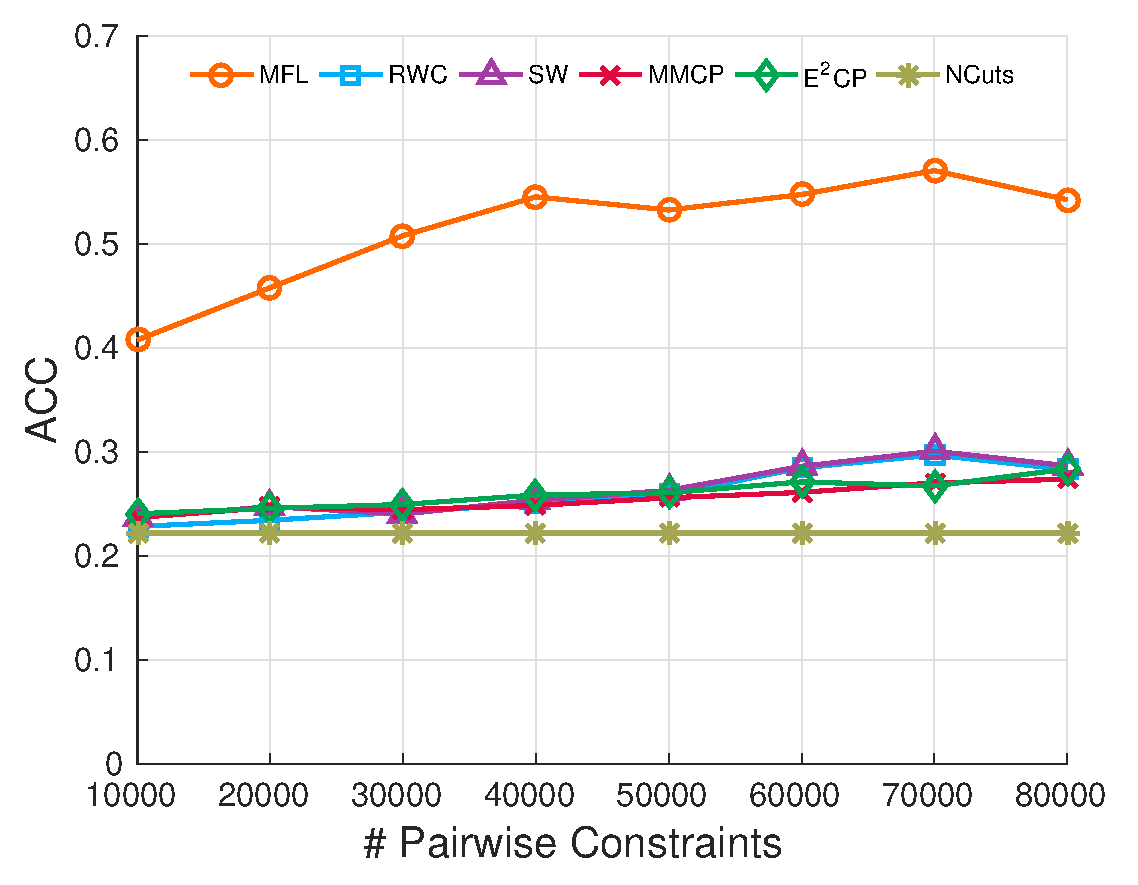
\includegraphics[width=0.49\textwidth]{chap3/voc_cn_16_acc.eps}}
                    \label{fig3:voc_cn_16_acc}
	\bisubcaptionbox{PASCAL VOC'07数据集上的NMI结果}%
					{NMI on  PASCAL VOC'07}
					[0.49\textwidth]{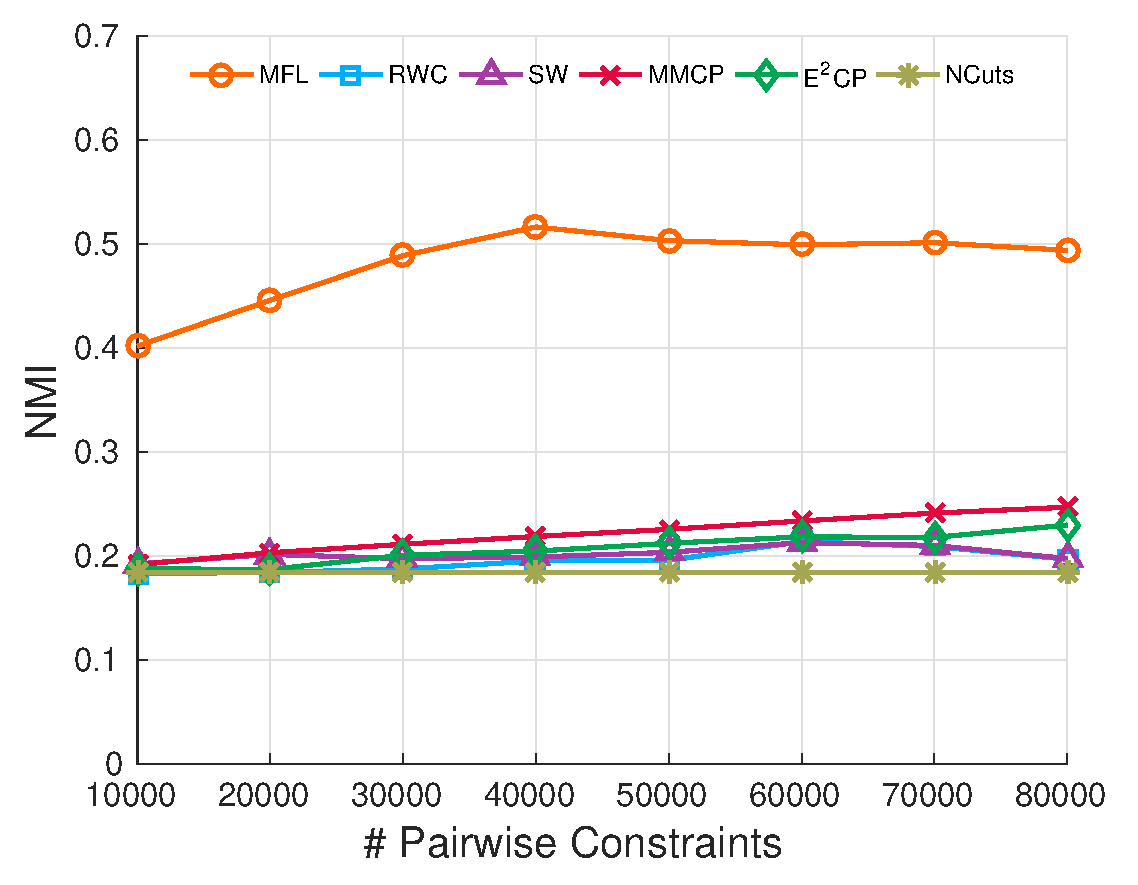
\includegraphics[width=0.49\textwidth]{chap3/voc_cn_16_nmi.eps}}
                    \label{fig3:voc_cn_16_nmi}
	\bicaption{在Corel 5k和PASCAL VOC'07数据集上,不同约束数量下采用16个模态的聚类效果}{Clustering performance of 16 modalities on Corel 5k and PASCAL VOC'07 with different numbers of  constraints}
	\label{fig3:cn_16}
\end{figure} 

实验中,除RWC中的$\gamma $之外,所有参数都有相同的参数选择标准。在RWC和MFL方法中传播参数$ \eta $如同MMCP和E$^2$CP一样都为$ 0.25 $。我们将$k$-NN近邻数量设置为$ k = \mathrm{Round}(\mathrm{log}_2(\frac{n}{c}))$,其中$ n $是数据实例的数量,$ c $是类别数。谱聚类中的特征嵌入维数为$ c + 1 $。

与Corel 5k数据集不同,PASCAL VOC'07数据集是为目标检测而提出的多标签数据集。该数据集中的许多数据样本都在真实标签中被标注了多个类别。我们在PASCAL VOC'07数据集上采用了一个标注技巧,而不是多标签聚类方法,以使性能与在Corel 5k上的聚类结果保持一致可比较。
我们将每个多标签数据样本复制多次以生成与其标签数量一样多的相同样本。然后,为每个副本分配一个标签。因此,带有$ t $个标签的数据样本将变成$ t $个分别仅带有一个标签的不同样本,尽管这些样本都有相同的的特征。使用这种多标签增强技巧后,性能测度ACC和NMI将始终小于1。因此,我们将评估结果除以理想化最优结果,以对评估分数进行归一化。

\subsection{性能评估与比较}
在本节中,我们报告并讨论了所提出的的MFL和RWC方法以及对照算法的聚类性能。为了将我们的方法与专门针对两种模态所设计的方法进行比较,我们设计了两种模态下的聚类实验。我们选择\textit{DenseSift}和\textit{tags}两种模态,并在表\ref{tab3:2modal}中展示了不同算法的聚类性能。我们选取成对约束总数的$0.08\%$作为观测到的成对约束信息,即在Corel 5k数据集上观察到的成对约束的数量为20,000对,在PASCAL VOC'07上观察到的约束的数量是80,000对。在以下实验中,我们采用相同数量的成对约束。从表\ref{tab3:2modal}中我们可以观察到,在Corel 5k数据集上,MFL和RWC表现出了相似的性能,并且胜过其他方法,而在PASCAL VOC'07上,SW方法的结果取得了最佳性能。这是由于\textit{DenseSift}和\textit{tags}两中特征的理想权重可能近似相等。但是,MFL和RWC方法的评估指标仍可与SW相媲美。此外,我们所提出的MFL并非专门针对两种模态情况设计,它旨在解决具有任何数量模态的权重学习问题。MFL仅为每个模态提供一个粗略的先验权重估计,权重估计的质量在很大程度上取决于观察到的约束矩阵$ {Y} $的质量。由于MFL是从约束矩阵$ {Y} $和稀疏相似性矩阵${W}_s $中学习先验权重,因此较少的模态将导致基矩阵$ {S} $存在大量的全零行,观察到的约束信息无法得到充分利用。如果我们有更多的模态或更多观察到的约束,则权重系数的预测将更加准确。这里需要注意的是,MSCP方法与UCP方法在约束传播后无法生成统一的相似性矩阵,即分别保留了经过约束传播的两个模态的相似性矩阵。因此在实验中我们对这两个相似性矩阵分别聚类,并在表\ref{tab3:2modal}种报告了聚类结果的平均值。

此外,我们在更多的模态上进行了的实验,并选择了三种不同的情况:3、8和16种模态。 在3种模态的情况下,我们将\textit{Lab}特征添加到前文所述的2种模态情况下。在8种模态的实验中,我们采用的特征为:\textit{DenseSift,Lab,tags,Hsv,Gist,RgbV3H1,HsvV3H1,HarrisSiftV3H1}。在16种模态的情况下,我们使用了INRIA特征数据集中的所有描述子。在表\ref{tab3:modal_corel}中我们展示了在Corel 5k数据集上的聚类结果,表\ref{tab3:modal_voc}显示了PASCAL VOC'07数据集上相应的聚类结果。从表\ref{tab3:modal_corel}和表\ref{tab3:modal_voc}中可以看出,随着模态数量的增加,提出的MFL算法的优越性变得愈加明显。当考虑到8或16种模态时,绝大多数对照方法都无法处理如此数量众多的模态。因此,我们能看出它们的性能出现明显的下降。

\begin{figure}[t]
    \centering
    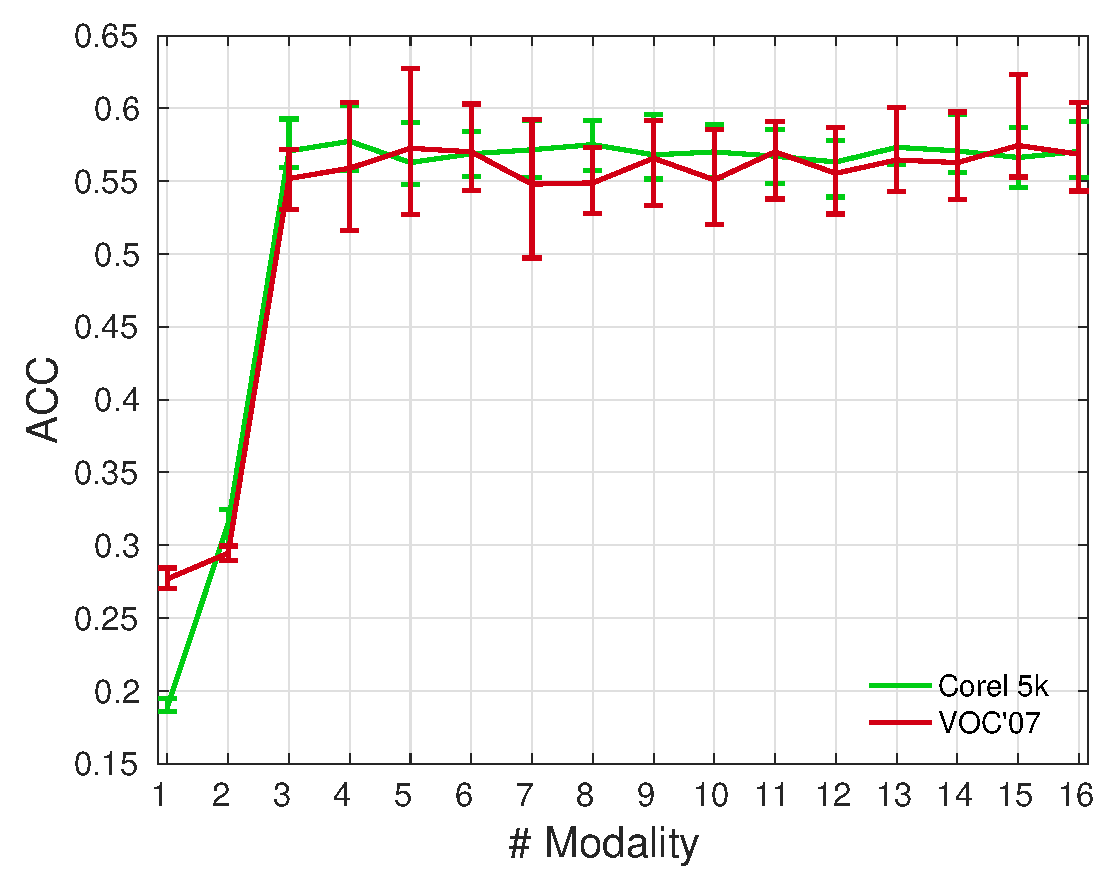
\includegraphics[width=0.49\textwidth]{chap3/corel5k_voc_1_16_acc.eps}
    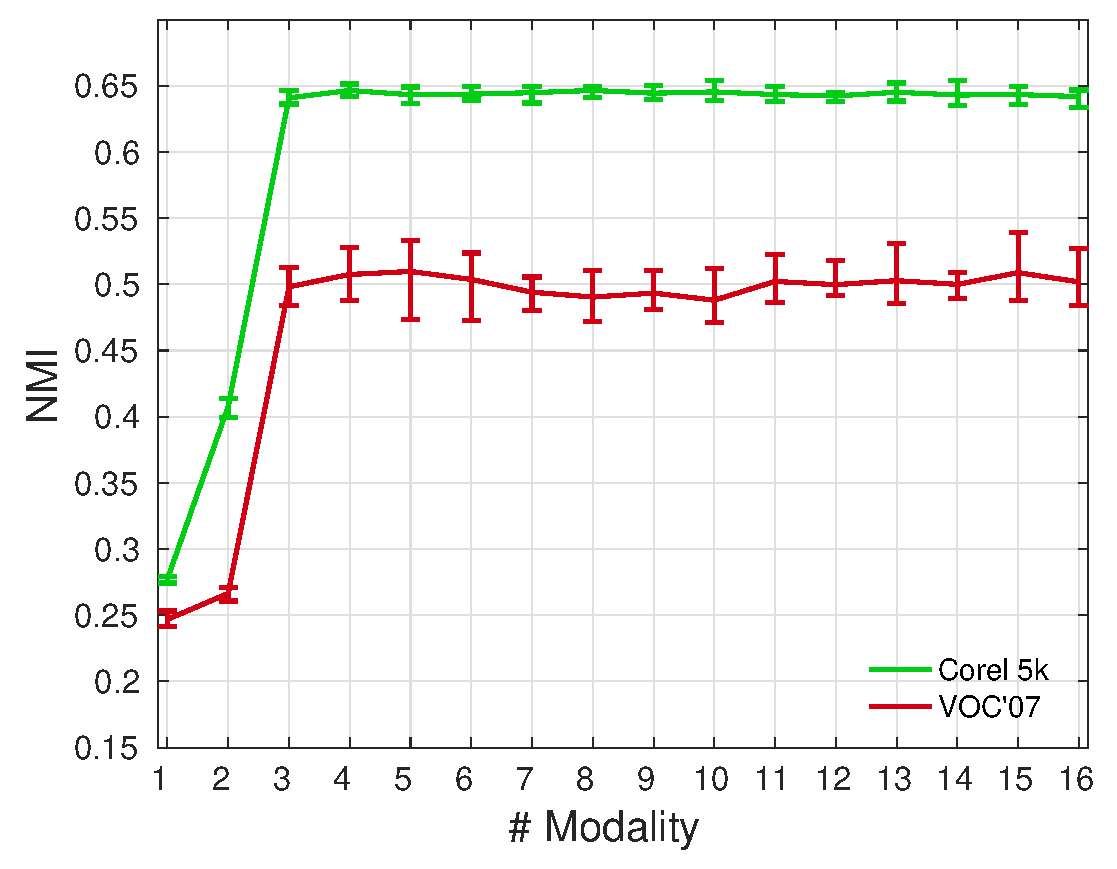
\includegraphics[width=0.49\textwidth]{chap3/corel5k_voc_1_16_nmi.eps}
	\bicaption{在不同数量模态上的聚类结果}{Clutering results with different number of modalities}
	\label{fig3:1_16}
\end{figure} 

在图\ref{fig3:cn}和图\ref{fig3:cn_16}中,我们展示了在3种和16种模态下,使用不同数量的成对约束的聚类效果。如前所述,由于MCMCP所需时间代价极大,本实验不涉及MCMCP方法,通过表\ref{tab3:2modal},表\ref{tab3:modal_corel}和表\ref{tab3:modal_voc}足以显示MCMCP的聚类性能。根据图\ref{fig3:cn}所显示的聚类结果,对于3种模态的情况,MFL方法在不同数量成对约束的设置下的聚类效果均优于其他方法,这种优势在图\ref{fig3:cn_16}所展示的实验结果中变得更加明显。


\begin{figure}[t]
	\centering
	\begin{subfigure}{0.49\textwidth}
		\centering
		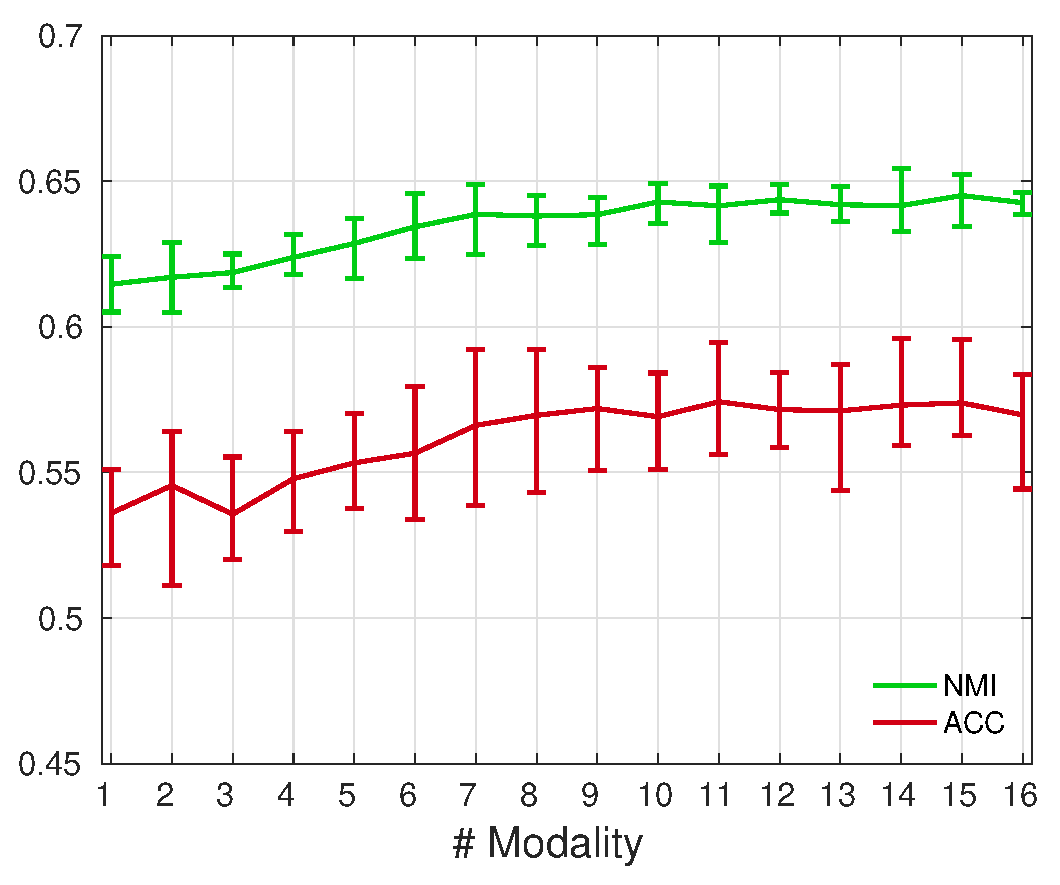
\includegraphics[width=\textwidth]{chap3/corel5k_1_16_acc_nmi_4.eps}
		\caption{}
		\label{fig3:1_16_acc_nmi_4}
	\end{subfigure}
	\begin{subfigure}{0.49\textwidth}
		\centering
		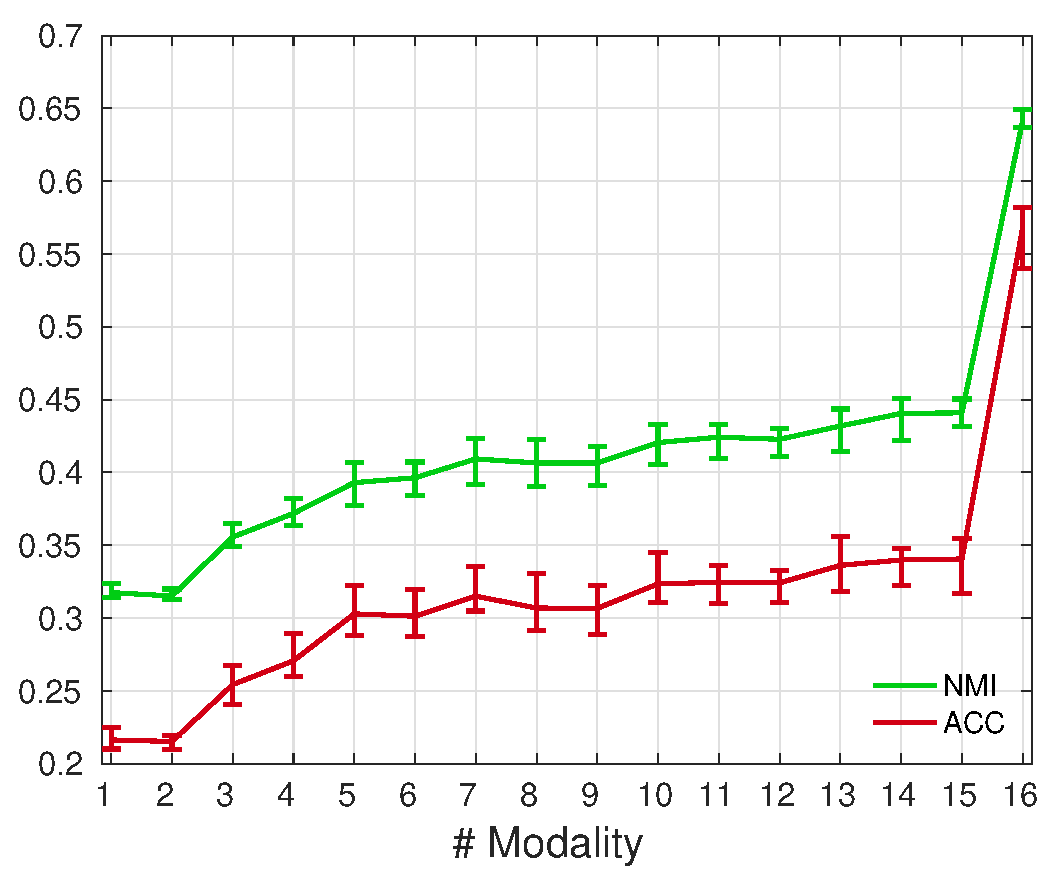
\includegraphics[width=\textwidth]{chap3/corel5k_1_16_acc_nmi_5.eps}
		\caption{}
		\label{fig3:1_16_acc_nmi_5}
    \end{subfigure}
    
	\centering
	\begin{subfigure}{0.49\textwidth}
		\centering
		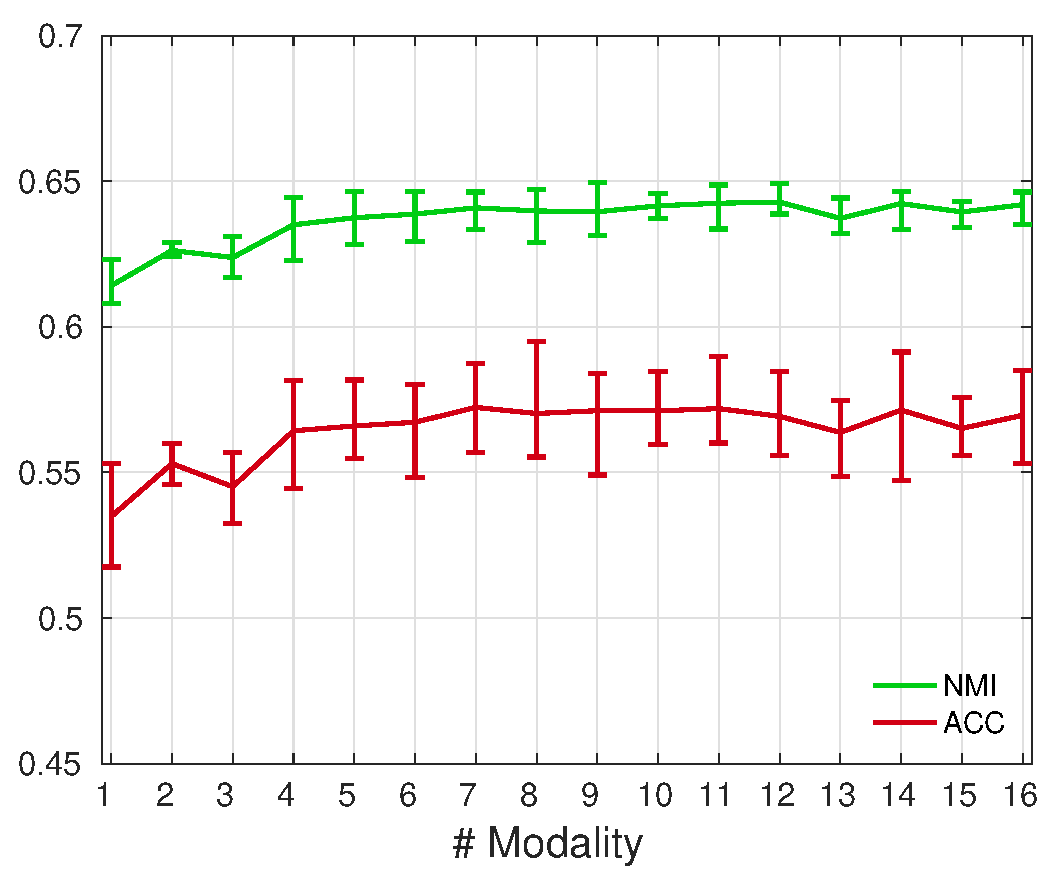
\includegraphics[width=\textwidth]{chap3/corel5k_1_16_acc_nmi_6.eps}
		\caption{}
		\label{fig3:1_16_acc_nmi_6}
	\end{subfigure}
	\begin{subfigure}{0.49\textwidth}
		\centering
		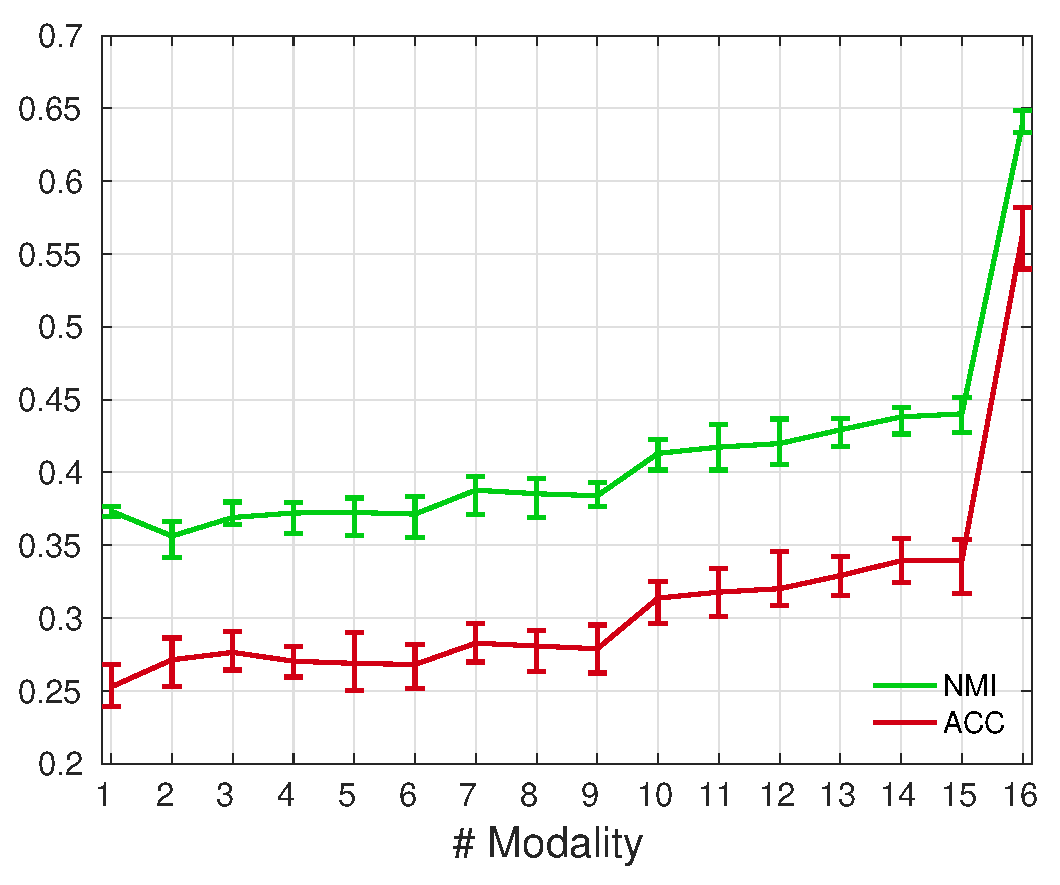
\includegraphics[width=\textwidth]{chap3/corel5k_1_16_acc_nmi_7.eps}
		\caption{}
		\label{fig3:1_16_acc_nmi_7}
	\end{subfigure}
	\bicaption{在Corel 5k数据集上不同模态顺序的聚类效果。a)以特征 \textit{tags} and \textit{HarrisHueV3H1}作为起始的模态序列;b)序列a)的逆序列;c)以特征 \textit{tags} and \textit{DenseSift}作为起始的模态序列;d)序列c)的逆序列}{Clutering results with different orders of modalities on Corel 5k. a) Modality sequence starts with \textit{tags} and \textit{HarrisHueV3H1}; b) Inverse order of a); c) Modality sequence starts with \textit{tags} and \textit{DenseSift}; d) Inverse order of c)}
    \label{fig3:1_16_more}
\end{figure}

正如在第\ref{sec3:dis}中所论述的,我们在图\ref{fig3:1_16}中研究了所提出的MFL算法的模态选择能力。在本实验中,通过将每种模态依次增添到MFL方法,以测试在不同数量模态的情况下MFL的聚类性能。选择的顺序为\textit{DenseSift,Lab,tags,Hsv,Gist,RgbV3H1,HsvV3H1,HarrisSiftV3H1,HarrisSift,HarrisSiftV3H1,DenseSiftV3H1,DenseHue,HarrisSift,HarrisHue,HarrisHueV3H1,Rgb}。可以注意到,当\textit{tags}特征被添加到MFL方法中时,聚类性能会显著地提高,然后效果近似达到饱和状态。这是因为文本描述特征本身包含了更多的具有判别性能力的信息,并且在\textit{tags}之后添加的特征只能提供一些冗余的信息。值得注意的是,每个模态都包含一些判别性信息以及噪声信息。如果新的模态无法提供非冗余信息,则额外引入的噪声将导致聚类性能下降。这也可以解释为什么大多数对照算法无法处理极其多种模态。与之相反的是,在MFL中,当不断增加模态数量时,权重的稀疏性将消除冗余的和不具有判别力的模态,从而保持鲁棒性。

为了进一步证明MFL算法可以帮助进行模态选择,仿照图\ref{fig3:1_16}的实验设置,以图\ref{fig3:1_16_more}来展示所提出的MFL在Corel 5k数据集上对于四种不同添加顺序的模态序列的聚类结果。图\ref{fig3:1_16_acc_nmi_4}所展示的模态添加顺序为\textit{tags,HarrisHueV3H1,Gist,DenseSiftV3H1,RgbV3H1,HsvV3H1,LabV3H1,DenseHueV3H1,HarrisSiftH3V1,Hsv,HarrisHue,DenseSift,HarrisSift,Lab,DenseHue,Rgb}。图\ref{fig3:1_16_acc_nmi_5}显示了图\ref{fig3:1_16_acc_nmi_4}中添加顺序的逆序的聚类结果,该序列以\textit{HarrisHueV3H1}和\textit{tags}作为结尾。图\ref{fig3:1_16_acc_nmi_6}的模态顺序为\textit{tags,DenseSift,Gist,LabV3H1,RgbV3H1,HsvV3H1,DenseSiftV3H1,DenseHueV3H1,HarrisSiftV3H1,Hsv,HarrisHue,HarrisHueV3H1,DenseHue,Rgb,HarrisSift,Lab}。图\ref{fig3:1_16_acc_nmi_7}显示了图\ref{fig3:1_16_acc_nmi_6}中添加顺序的逆序的聚类结果,该序列以\textit{DenseSift}和\textit{tags}结尾。可以注意到,在以\textit{tags}起始的图\ref{fig3:1_16_acc_nmi_4}和图\ref{fig3:1_16_acc_nmi_6}中,仅使用一种或两种模态信息,所取得的聚类性能已经非常出色。这是因为\textit{tags}是文本描述信息,比视觉描述更具有判别性。在向序列中添加更多的模态后,由于来自视觉描述特征的附加信息,实验结果得到了$2\%$的性能改进。而在多数实际应用中,文本描述是一种从用户处收集代价较高的特征。我们更进一步地在图\ref{fig3:1_16_acc_nmi_5}和图\ref{fig3:1_16_acc_nmi_7}中展示以\textit{tags}作为结束地模态序列的聚类效果。尽管\textit{tags}能够产生可观的性能改进,但是聚类性能依然收益于持续增加的视觉特征数量。如果没有文本描述,在仅使15种模态的情况下,所提出的MFL算法在仅用利用一种或两种模态的基础上,大约可提高$10\%$的聚类性能。

\section{本章小结}
在本章中,我们将多标签传播中广泛使用的RWC方法通过近似的方式引入了多模态约束传播问题。更进一步地,本章提出了一种在多模态约束传播中的新颖的融合学习方法,称为多模态融合学习(Multi-modal Fusion Learning,MFL)。MFL方法从所观察到的成对约束的重建损失以及传播过程中学习模态的相似性融合。此外,本章还讨论了不同的算法在极多数量的模态下的承压能力,并通过大量实验结果证明了所提出方法的优越性。